
%% bare_conf.tex
%% V1.4a
%% 2014/09/17
%% by Michael Shell
%% See:
%% http://www.michaelshell.org/
%% for current contact information.
%%
%% This is a skeleton file demonstrating the use of IEEEtran.cls
%% (requires IEEEtran.cls version 1.8a or later) with an IEEE
%% conference paper.
%%
%% Support sites:
%% http://www.michaelshell.org/tex/ieeetran/
%% http://www.ctan.org/tex-archive/macros/latex/contrib/IEEEtran/
%% and
%% http://www.ieee.org/

%%*************************************************************************
%% Legal Notice:
%% This code is offered as-is without any warranty either expressed or
%% implied; without even the implied warranty of MERCHANTABILITY or
%% FITNESS FOR A PARTICULAR PURPOSE! 
%% User assumes all risk.
%% In no event shall IEEE or any contributor to this code be liable for
%% any damages or losses, including, but not limited to, incidental,
%% consequential, or any other damages, resulting from the use or misuse
%% of any information contained here.
%%
%% All comments are the opinions of their respective authors and are not
%% necessarily endorsed by the IEEE.
%%
%% This work is distributed under the LaTeX Project Public License (LPPL)
%% ( http://www.latex-project.org/ ) version 1.3, and may be freely used,
%% distributed and modified. A copy of the LPPL, version 1.3, is included
%% in the base LaTeX documentation of all distributions of LaTeX released
%% 2003/12/01 or later.
%% Retain all contribution notices and credits.
%% ** Modified files should be clearly indicated as such, including  **
%% ** renaming them and changing author support contact information. **
%%
%% File list of work: IEEEtran.cls, IEEEtran_HOWTO.pdf, bare_adv.tex,
%%                    bare_conf.tex, bare_jrnl.tex, bare_conf_compsoc.tex,
%%                    bare_jrnl_compsoc.tex, bare_jrnl_transmag.tex
%%*************************************************************************


% *** Authors should verify (and, if needed, correct) their LaTeX system  ***
% *** with the testflow diagnostic prior to trusting their LaTeX platform ***
% *** with production work. IEEE's font choices and paper sizes can       ***
% *** trigger bugs that do not appear when using other class files.       ***                          ***
% The testflow support page is at:
% http://www.michaelshell.org/tex/testflow/



\documentclass[conference]{Trabalho_2}
\usepackage{graphicx, url, epsfig, subfigure, caption, subcaption}
\usepackage{amsmath, amscd, amsthm, amsxtra}
\usepackage[T1]{fontenc}
\usepackage[brazil]{babel}   
\usepackage[latin1]{inputenc}
\usepackage{listings}
\usepackage{color}
\usepackage{verbatim}

% Some Computer Society conferences also require the compsoc mode option,
% but others use the standard conference format.
%
% If IEEEtran.cls has not been installed into the LaTeX system files,
% manually specify the path to it like:
% \documentclass[conference]{../sty/IEEEtran}





% Some very useful LaTeX packages include:2
% (uncomment the ones you want to load)


% *** MISC UTILITY PACKAGES ***
%
%\usepackage{ifpdf}
% Heiko Oberdiek's ifpdf.sty is very useful if you need conditional
% compilation based on whether the output is pdf or dvi.
% usage:
% \ifpdf
%   % pdf code
% \else
%   % dvi code
% \fi
% The latest version of ifpdf.sty can be obtained from:
% http://www.ctan.org/tex-archive/macros/latex/contrib/oberdiek/
% Also, note that IEEEtran.cls V1.7 and later provides a builtin
% \ifCLASSINFOpdf conditional that works the same way.
% When switching from latex to pdflatex and vice-versa, the compiler may
% have to be run twice to clear warning/error messages.






% *** CITATION PACKAGES ***
%
%\usepackage{cite}
% cite.sty was written by Donald Arseneau
% V1.6 and later of IEEEtran pre-defines the format of the cite.sty package
% \cite{} output to follow that of IEEE. Loading the cite package will
% result in citation numbers being automatically sorted and properly
% "compressed/ranged". e.g., [1], [9], [2], [7], [5], [6] without using
% cite.sty will become [1], [2], [5]--[7], [9] using cite.sty. cite.sty's
% \cite will automatically add leading space, if needed. Use cite.sty's
% noadjust option (cite.sty V3.8 and later) if you want to turn this off
% such as if a citation ever needs to be enclosed in parenthesis.
% cite.sty is already installed on most LaTeX systems. Be sure and use
% version 5.0 (2009-03-20) and later if using hyperref.sty.
% The latest version can be obtained at:
% http://www.ctan.org/tex-archive/macros/latex/contrib/cite/
% The documentation is contained in the cite.sty file itself.






% *** GRAPHICS RELATED PACKAGES ***
%
\ifCLASSINFOpdf
  % \usepackage[pdftex]{graphicx}
  % declare the path(s) where your graphic files are
  % \graphicspath{{../pdf/}{../jpeg/}}
  % and their extensions so you won't have to specify these with
  % every instance of \includegraphics
  % \DeclareGraphicsExtensions{.pdf,.jpeg,.png}
\else
  % or other class option (dvipsone, dvipdf, if not using dvips). graphicx
  % will default to the driver specified in the system graphics.cfg if no
  % driver is specified.
  % \usepackage[dvips]{graphicx}
  % declare the path(s) where your graphic files are
  % \graphicspath{{../eps/}}
  % and their extensions so you won't have to specify these with
  % every instance of \includegraphics
  % \DeclareGraphicsExtensions{.eps}
\fi
% graphicx was written by David Carlisle and Sebastian Rahtz. It is
% required if you want graphics, photos, etc. graphicx.sty is already
% installed on most LaTeX systems. The latest version and documentation
% can be obtained at: 
% http://www.ctan.org/tex-archive/macros/latex/required/graphics/
% Another good source of documentation is "Using Imported Graphics in
% LaTeX2e" by Keith Reckdahl which can be found at:
% http://www.ctan.org/tex-archive/info/epslatex/
%
% latex, and pdflatex in dvi mode, support graphics in encapsulated
% postscript (.eps) format. pdflatex in pdf mode supports graphics
% in .pdf, .jpeg, .png and .mps (metapost) formats. Users should ensure
% that all non-photo figures use a vector format (.eps, .pdf, .mps) and
% not a bitmapped formats (.jpeg, .png). IEEE frowns on bitmapped formats
% which can result in "jaggedy"/blurry rendering of lines and letters as
% well as large increases in file sizes.
%
% You can find documentation about the pdfTeX application at:
% http://www.tug.org/applications/pdftex





% *** MATH PACKAGES ***
%
%\usepackage[cmex10]{amsmath}
% A popular package from the American Mathematical Society that provides
% many useful and powerful commands for dealing with mathematics. If using
% it, be sure to load this package with the cmex10 option to ensure that
% only type 1 fonts will utilized at all point sizes. Without this option,
% it is possible that some math symbols, particularly those within
% footnotes, will be rendered in bitmap form which will result in a
% document that can not be IEEE Xplore compliant!
%
% Also, note that the amsmath package sets \interdisplaylinepenalty to 10000
% thus preventing page breaks from occurring within multiline equations. Use:
%\interdisplaylinepenalty=2500
% after loading amsmath to restore such page breaks as IEEEtran.cls normally
% does. amsmath.sty is already installed on most LaTeX systems. The latest
% version and documentation can be obtained at:
% http://www.ctan.org/tex-archive/macros/latex/required/amslatex/math/





% *** SPECIALIZED LIST PACKAGES ***
%
%\usepackage{algorithmic}
% algorithmic.sty was written by Peter Williams and Rogerio Brito.
% This package provides an algorithmic environment fo describing algorithms.
% You can use the algorithmic environment in-text or within a figure
% environment to provide for a floating algorithm. Do NOT use the algorithm
% floating environment provided by algorithm.sty (by the same authors) or
% algorithm2e.sty (by Christophe Fiorio) as IEEE does not use dedicated
% algorithm float types and packages that provide these will not provide
% correct IEEE style captions. The latest version and documentation of
% algorithmic.sty can be obtained at:
% http://www.ctan.org/tex-archive/macros/latex/contrib/algorithms/
% There is also a support site at:
% http://algorithms.berlios.de/index.html
% Also of interest may be the (relatively newer and more customizable)
% algorithmicx.sty package by Szasz Janos:
% http://www.ctan.org/tex-archive/macros/latex/contrib/algorithmicx/




% *** ALIGNMENT PACKAGES ***
%
%\usepackage{array}
% Frank Mittelbach's and David Carlisle's array.sty patches and improves
% the standard LaTeX2e array and tabular environments to provide better
% appearance and additional user controls. As the default LaTeX2e table
% generation code is lacking to the point of almost being broken with
% respect to the quality of the end results, all users are strongly
% advised to use an enhanced (at the very least that provided by array.sty)
% set of table tools. array.sty is already installed on most systems. The
% latest version and documentation can be obtained at:
% http://www.ctan.org/tex-archive/macros/latex/required/tools/


% IEEEtran contains the IEEEeqnarray family of commands that can be used to
% generate multiline equations as well as matrices, tables, etc., of high
% quality.




% *** SUBFIGURE PACKAGES ***
%\ifCLASSOPTIONcompsoc
%  \usepackage[caption=false,font=normalsize,labelfont=sf,textfont=sf]{subfig}
%\else
%  \usepackage[caption=false,font=footnotesize]{subfig}
%\fi
% subfig.sty, written by Steven Douglas Cochran, is the modern replacement
% for subfigure.sty, the latter of which is no longer maintained and is
% incompatible with some LaTeX packages including fixltx2e. However,
% subfig.sty requires and automatically loads Axel Sommerfeldt's caption.sty
% which will override IEEEtran.cls' handling of captions and this will result
% in non-IEEE style figure/table captions. To prevent this problem, be sure
% and invoke subfig.sty's "caption=false" package option (available since
% subfig.sty version 1.3, 2005/06/28) as this is will preserve IEEEtran.cls
% handling of captions.
% Note that the Computer Society format requires a larger sans serif font
% than the serif footnote size font used in traditional IEEE formatting
% and thus the need to invoke different subfig.sty package options depending
% on whether compsoc mode has been enabled.
%
% The latest version and documentation of subfig.sty can be obtained at:
% http://www.ctan.org/tex-archive/macros/latex/contrib/subfig/




% *** FLOAT PACKAGES ***
%
%\usepackage{fixltx2e}
% fixltx2e, the successor to the earlier fix2col.sty, was written by
% Frank Mittelbach and David Carlisle. This package corrects a few problems
% in the LaTeX2e kernel, the most notable of which is that in current
% LaTeX2e releases, the ordering of single and double column floats is not
% guaranteed to be preserved. Thus, an unpatched LaTeX2e can allow a
% single column figure to be placed prior to an earlier double column
% figure. The latest version and documentation can be found at:
% http://www.ctan.org/tex-archive/macros/latex/base/


%\usepackage{stfloats}
% stfloats.sty was written by Sigitas Tolusis. This package gives LaTeX2e
% the ability to do double column floats at the bottom of the page as well
% as the top. (e.g., "\begin{figure*}[!b]" is not normally possible in
% LaTeX2e). It also provides a command:
%\fnbelowfloat
% to enable the placement of footnotes below bottom floats (the standard
% LaTeX2e kernel puts them above bottom floats). This is an invasive package
% which rewrites many portions of the LaTeX2e float routines. It may not work
% with other packages that modify the LaTeX2e float routines. The latest
% version and documentation can be obtained at:
% http://www.ctan.org/tex-archive/macros/latex/contrib/sttools/
% Do not use the stfloats baselinefloat ability as IEEE does not allow
% \baselineskip to stretch. Authors submitting work to the IEEE should note
% that IEEE rarely uses double column equations and that authors should try
% to avoid such use. Do not be tempted to use the cuted.sty or midfloat.sty
% packages (also by Sigitas Tolusis) as IEEE does not format its papers in
% such ways.
% Do not attempt to use stfloats with fixltx2e as they are incompatible.
% Instead, use Morten Hogholm'a dblfloatfix which combines the features
% of both fixltx2e and stfloats:
%
% \usepackage{dblfloatfix}
% The latest version can be found at:
% http://www.ctan.org/tex-archive/macros/latex/contrib/dblfloatfix/




% *** PDF, URL AND HYPERLINK PACKAGES ***
%
%\usepackage{url}
% url.sty was written by Donald Arseneau. It provides better support for
% handling and breaking URLs. url.sty is already installed on most LaTeX
% systems. The latest version and documentation can be obtained at:
% http://www.ctan.org/tex-archive/macros/latex/contrib/url/
% Basically, \url{my_url_here}.




% *** Do not adjust lengths that control margins, column widths, etc. ***
% *** Do not use packages that alter fonts (such as pslatex).         ***
% There should be no need to do such things with IEEEtran.cls V1.6 and later.
% (Unless specifically asked to do so by the journal or conference you plan
% to submit to, of course. )


% correct bad hyphenation here
\hyphenation{op-tical net-works semi-conduc-tor}


\begin{document}
%
% paper title
% Titles are generally capitalized except for words such as a, an, and, as,
% at, but, by, for, in, nor, of, on, or, the, to and up, which are usually
% not capitalized unless they are the first or last word of the title.
% Linebreaks \\ can be used within to get better formatting as desired.
% Do not put math or special symbols in the title.
\title{Morfologia Matem\'atica e Segmenta\c{c}\~ao}


% author names and affiliations
% use a multiple column layout for up to three different
% affiliations
\author{\IEEEauthorblockN{Rodrigo Ferreira Guimar\~aes}
\IEEEauthorblockA{Departamento de Ci\^encia de Computa\c{c}\~ao e Faculdade de Tecnologia\\
Universidade de Bras\'ilia, Bras\'ilia\\
Email: rodrigofegui@aluno.unb.br\\
Matr\'icula: 14/0170740}
}

% conference papers do not typically use \thanks and this command
% is locked out in conference mode. If really needed, such as for
% the acknowledgment of grants, issue a \IEEEoverridecommandlockouts
% after \documentclass

% for over three affiliations, or if they all won't fit within the width
% of the page, use this alternative format:
% 
%\author{\IEEEauthorblockN{Michael Shell\IEEEauthorrefmark{1},
%Homer Simpson\IEEEauthorrefmark{2},
%James Kirk\IEEEauthorrefmark{3}, 
%Montgomery Scott\IEEEauthorrefmark{3} and
%Eldon Tyrell\IEEEauthorrefmark{4}}
%\IEEEauthorblockA{\IEEEauthorrefmark{1}School of Electrical and Computer Engineering\\
%Georgia Institute of Technology,
%Atlanta, Georgia 30332--0250\\ Email: see http://www.michaelshell.org/contact.html}
%\IEEEauthorblockA{\IEEEauthorrefmark{2}Twentieth Century Fox, Springfield, USA\\
%Email: homer@thesimpsons.com}
%\IEEEauthorblockA{\IEEEauthorrefmark{3}Starfleet Academy, San Francisco, California 96678-2391\\
%Telephone: (800) 555--1212, Fax: (888) 555--1212}
%\IEEEauthorblockA{\IEEEauthorrefmark{4}Tyrell Inc., 123 Replicant Street, Los Angeles, California 90210--4321}}




% use for special paper notices
%\IEEEspecialpapernotice{(Invited Paper)}




% make the title area
\maketitle

% As a general rule, do not put math, special symbols or citations
% in the abstract
%\begin{abstract}
%O resumo vem aqui.
%\end{abstract}

% no keywords




% For peer review papers, you can put extra information on the cover
% page as needed:
% \ifCLASSOPTIONpeerreview
% \begin{center} \bfseries EDICS Category: 3-BBND \end{center}
% \fi
%
% For peerreview papers, this IEEEtran command inserts a page break and
% creates the second title. It will be ignored for other modes.
\IEEEpeerreviewmaketitle



\section{Introdu\c{c}\~ao}
Este trabalho visa fixar os conceitos relativos a morfologia matem\'atica e segmenta\c{c}\~ao. Para atingir tal objetivo foram consideradas tr\^es problemas:~\textbf{a)} uma imagem de circuito impresso que deveria ser manipulada de forma a obter o n\'umero de buracos e seus di\^ametros em~\textit{pixels};~\textbf{b)} uma imagem de fundo borrado e com n\'umeros aleat\'orios, como uma camada superior, que deveria ser manipulada de forma a obter uma imagem de fundo branco e texto preto; e por \'ultimo,~\textbf{c)} uma imagem com c\'elulas que deveria ser manipulada de forma a obter uma imagem de fundo branco e c\'elulas pretas.

 
\hfill 26 de Outubro, 2015


% An example of a floating figure using the graphicx package.
% Note that \label must occur AFTER (or within) \caption.
% For figures, \caption should occur after the \includegraphics.
% Note that IEEEtran v1.7 and later has special internal code that
% is designed to preserve the operation of \label within \caption
% even when the captionsoff option is in effect. However, because
% of issues like this, it may be the safest practice to put all your
% \label just after \caption rather than within \caption{}.
%
% Reminder: the "draftcls" or "draftclsnofoot", not "draft", class
% option should be used if it is desired that the figures are to be
% displayed while in draft mode.
%
%\begin{figure}[!t]
%\centering
%\includegraphics[width=2.5in]{myfigure}
% where an .eps filename suffix will be assumed under latex, 
% and a .pdf suffix will be assumed for pdflatex; or what has been declared
% via \DeclareGraphicsExtensions.
%\caption{Simulation results for the network.}
%\label{fig_sim}
%\end{figure}

% Note that IEEE typically puts floats only at the top, even when this
% results in a large percentage of a column being occupied by floats.


% An example of a double column floating figure using two subfigures.
% (The subfig.sty package must be loaded for this to work.)
% The subfigure \label commands are set within each subfloat command,
% and the \label for the overall figure must come after \caption.
% \hfil is used as a separator to get equal spacing.
% Watch out that the combined width of all the subfigures on a 
% line do not exceed the text width or a line break will occur.
%
%\begin{figure*}[!t]
%\centering
%\subfloat[Case I]{\includegraphics[width=2.5in]{box}%
%\label{fig_first_case}}
%\hfil
%\subfloat[Case II]{\includegraphics[width=2.5in]{box}%
%\label{fig_second_case}}
%\caption{Simulation results for the network.}
%\label{fig_sim}
%\end{figure*}
%
% Note that often IEEE papers with subfigures do not employ subfigure
% captions (using the optional argument to \subfloat[]), but instead will
% reference/describe all of them (a), (b), etc., within the main caption.
% Be aware that for subfig.sty to generate the (a), (b), etc., subfigure
% labels, the optional argument to \subfloat must be present. If a
% subcaption is not desired, just leave its contents blank,
% e.g., \subfloat[].


% An example of a floating table. Note that, for IEEE style tables, the
% \caption command should come BEFORE the table and, given that table
% captions serve much like titles, are usually capitalized except for words
% such as a, an, and, as, at, but, by, for, in, nor, of, on, or, the, to
% and up, which are usually not capitalized unless they are the first or
% last word of the caption. Table text will default to \footnotesize as
% IEEE normally uses this smaller font for tables.
% The \label must come after \caption as always.
%
%\begin{table}[!t]
%% increase table row spacing, adjust to taste
%\renewcommand{\arraystretch}{1.3}
% if using array.sty, it might be a good idea to tweak the value of
% \extrarowheight as needed to properly center the text within the cells
%\caption{An Example of a Table}
%\label{table_example}
%\centering
%% Some packages, such as MDW tools, offer better commands for making tables
%% than the plain LaTeX2e tabular which is used here.
%\begin{tabular}{|c||c|}
%\hline
%One & Two\\
%\hline
%Three & Four\\
%\hline
%\end{tabular}
%\end{table}


% Note that the IEEE does not put floats in the very first column
% - or typically anywhere on the first page for that matter. Also,
% in-text middle ("here") positioning is typically not used, but it
% is allowed and encouraged for Computer Society conferences (but
% not Computer Society journals). Most IEEE journals/conferences use
% top floats exclusively. 
% Note that, LaTeX2e, unlike IEEE journals/conferences, places
% footnotes above bottom floats. This can be corrected via the
% \fnbelowfloat command of the stfloats package.


\section{Embasamento Te\'orico}
Para que haja um correto entendimento sobre o desenvolvimento deste projeto \'e importante abordar alguns aspectos relevantes, como as defini\c{c}\~oes: de uma imagem; das rela\c{c}\c{c}\~oes b\'asicas entre~\textit{pixels}: adjac\^encia, conectividade, regi\~ao e contorno; opera\c{c}\~oes morfol\'oligas; segmenta\c{c}\~ao, dentre outras coisas

\subsection{Imagem e~\textit{Pixels}}
Uma imagem pode ser definida como uma fun\c{c}\~ao bidimensional do tipo $f(x,y)$, onde $x$ e $y$ s\~ao as coordenadas espaciais e a amplitude de $f$ em qualquer ponto de coordenadas $(x,y)$ \'e denominado de intensidade da imagem naquele ponto. Quando $x$, $y$ e $f$ s\~ao valores~\textit{finitos} e~\textit{discretos}, a imagem \'e denominada imagem digital, tendo esta signific\^ancia aos computadores digitais. Um dado elemento com coordenadas $(x,y)$ e intensidade $f$ \'e denominado de~\textit{pixel}~(picture element ou, em portugu\^es, elemento de imagem), dessa forma, entende-se que uma imagem \'e constituida por um ou mais~\textit{pixels}.

Para a manipula\c{c}\~ao dos~\textit{pixels} \'e necess\'ario saber as rela\c{c}\~oes b\'asicas entre eles, como, por exemplo, a vizinhan\c{c}a. Os conceito a serem apresentados consideram uma imagem em n\'ivel de cinza.

Cada~\textit{pixel} $p$ pode possui tr\^es tipos de vizinhan\c{c}a, semelhantes a Rosa-dos-Ventos da Figura~\ref{fig:rosadosventos}:~\textit{vizinhan\c{c}a de 4},~\textit{vizinhan\c{c}a diagonal} e~\textit{vizinhan\c{c}a de 8}; onde para o primeiro, denonato por $N_4$(p), s\~ao considerados os quatro vizinhos horizontais e verticais, seguindo as orienta\c{c}\~oes~\textit{N-S-L-O} da Rosa-dos-Ventos; para o segundo, denonato por $N_D$(p), s\~ao considerados os vizinhos das diagonais, seguindo as orienta\c{c}\~oes~\textit{NE-SE-SO-NO}; enquanto que o terceiro tipo, denonato por $N_8$(p), \'e a jun\c{c}\~ao dos dois anteriores.

\begin{figure}[!t]
  \centering
  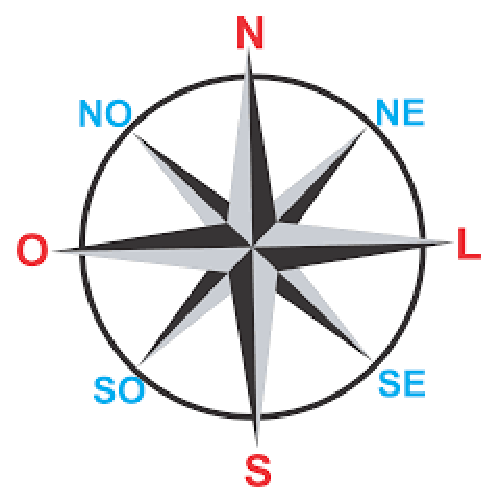
\includegraphics[width = 4.5 cm]{rosadosventos}
  \caption{Sinaliza\c{c}\~ao dos sentido cardeias da Rosa-dos-Ventos. Fonte~\cite{rosadosventos}.}
  \label{fig:rosadosventos}
\end{figure}

\subsection{Rela\c{c}\~oes B\'asicas entre~\textit{Pixels}}
Com o conceito de vizinhan\c{c}a constru\'ido \'e poss\'ivel entender o conceito de adjac\^encia, entre dois~\textit{pixels} $p$ e $q$, que, tamb\'em, possui tr\^es tipos, sendo eles:

\begin{itemize}
 \item \textbf{Adjac\^encia de 4}: os dois~\textit{pixels} s\~ao adjacentes de 4 se ambos possuirem o mesmo n\'ivel de cinza e se $q$ est\'a na $N_4$(p);
 \item \textbf{Adjac\^encia de 8}: os dois~\textit{pixels} s\~ao adjacentes de 4 se ambos possuirem o mesmo n\'ivel de cinza e se $q$ est\'a na $N_8$(p);
 \item \textbf{Adjac\^encia de~\textit{m}}: os dois~\textit{pixels} s\~ao adjacentes de~\textit{m} se ambos possuirem o mesmo n\'ivel de cinza e se respeitarem as condi\c{c}\~oes:~\textbf{a)} $q$ est\'a na $N_4$(p) ou~\textbf{b)} $q$ est\'a na $N_D$(p) e n\~ao h\'a interse\c{c}\~ao entre a $N_4$(p) e $N_4$(q). 
\end{itemize}

Considerando um subconjunto $S$ de imagem, dois~\textit{pixels} pertencentes a $S$ s\~ao conectados, considerando um dos crit\'erios de adjac\^encia, caso exista um caminho entre eles que tamb\'em perten\c{c}a a $S$. Para qualquer~\textit{pixel} $p$ em $S$, o conjunto de~\textit{pixels} que proporciona a uni\~ao a $q$ \'e denominado de~\textit{conjunto conectado}. Caso $q$ seja adjacente a $p$, este \'e chamado de~\textit{componente conectado}.

Uma regi\~ao $R$ \'e definida como um conjunto conectado e o contorno $C$ de $R$ \'e definido como sendo os~\textit{pixels} que possuem vizinhos que tanto pertencem $R$ como n\~ao pertencente.

\subsection{Opera\c{c}\~oes Morfol\'ogicas}
A morfologia, geralmente, \'e considerada apenas como uma especializa\c{c}\~ao da biologia que trabalha com a forma e a estrutura dos seres vivos. Al\'em desse conceito, h\'a a morfologia matem\'atica que estuda o processamento e an\'alise de estruturas geom\'etricas. Com esses, tem que para o processamento de imagens \'e aplicado a morfologia matem\'atica, pois dessa forma \'e realizada a extra\c{c}\~ao de regi\~oes de uma imagem, representa\c{c}\~ao e descri\c{c}\~ao das formas de uma determinada regi\~ao.

Dessa forma, considerando imagens bin\'arias, tem-se algunas opera\c{c}\~oes que foram utilizadas para a realiza\c{c}\~ao desde projeto, sendo elas: eros\~ao; dilata\c{c}\~ao; fechamento;~\textit{top-hat} e~\textit{bottom-hat}; e~\textit{watershed}, sendo elas explicadas a seguir.

\subsubsection{Eros\~ao}
A eros\~ao \'e definida como sendo:
$$ A \ominus B  = \{z \mid (B)_z \subseteq A\},$$
ou seja, a eros\~ao de $A$ por $B$ \'e o conjunto de todos os pontos $z$, tal que $B$ transladado de $z$ est\'a contido em $A$, como demonstrado na Figura~\ref{fig:erosao} ($B$ \'e chamado~\textit{elemento estruturante}). Dessa forma ao considerar que $B$ n\~ao tem elementos comuns com o fundo \'e poss\'ivel reescrever como sendo:
$$ A \ominus B  = \{z \mid (B)_z \cap A{^c} = \emptyset \}.$$

\begin{figure}[]
  \centering
  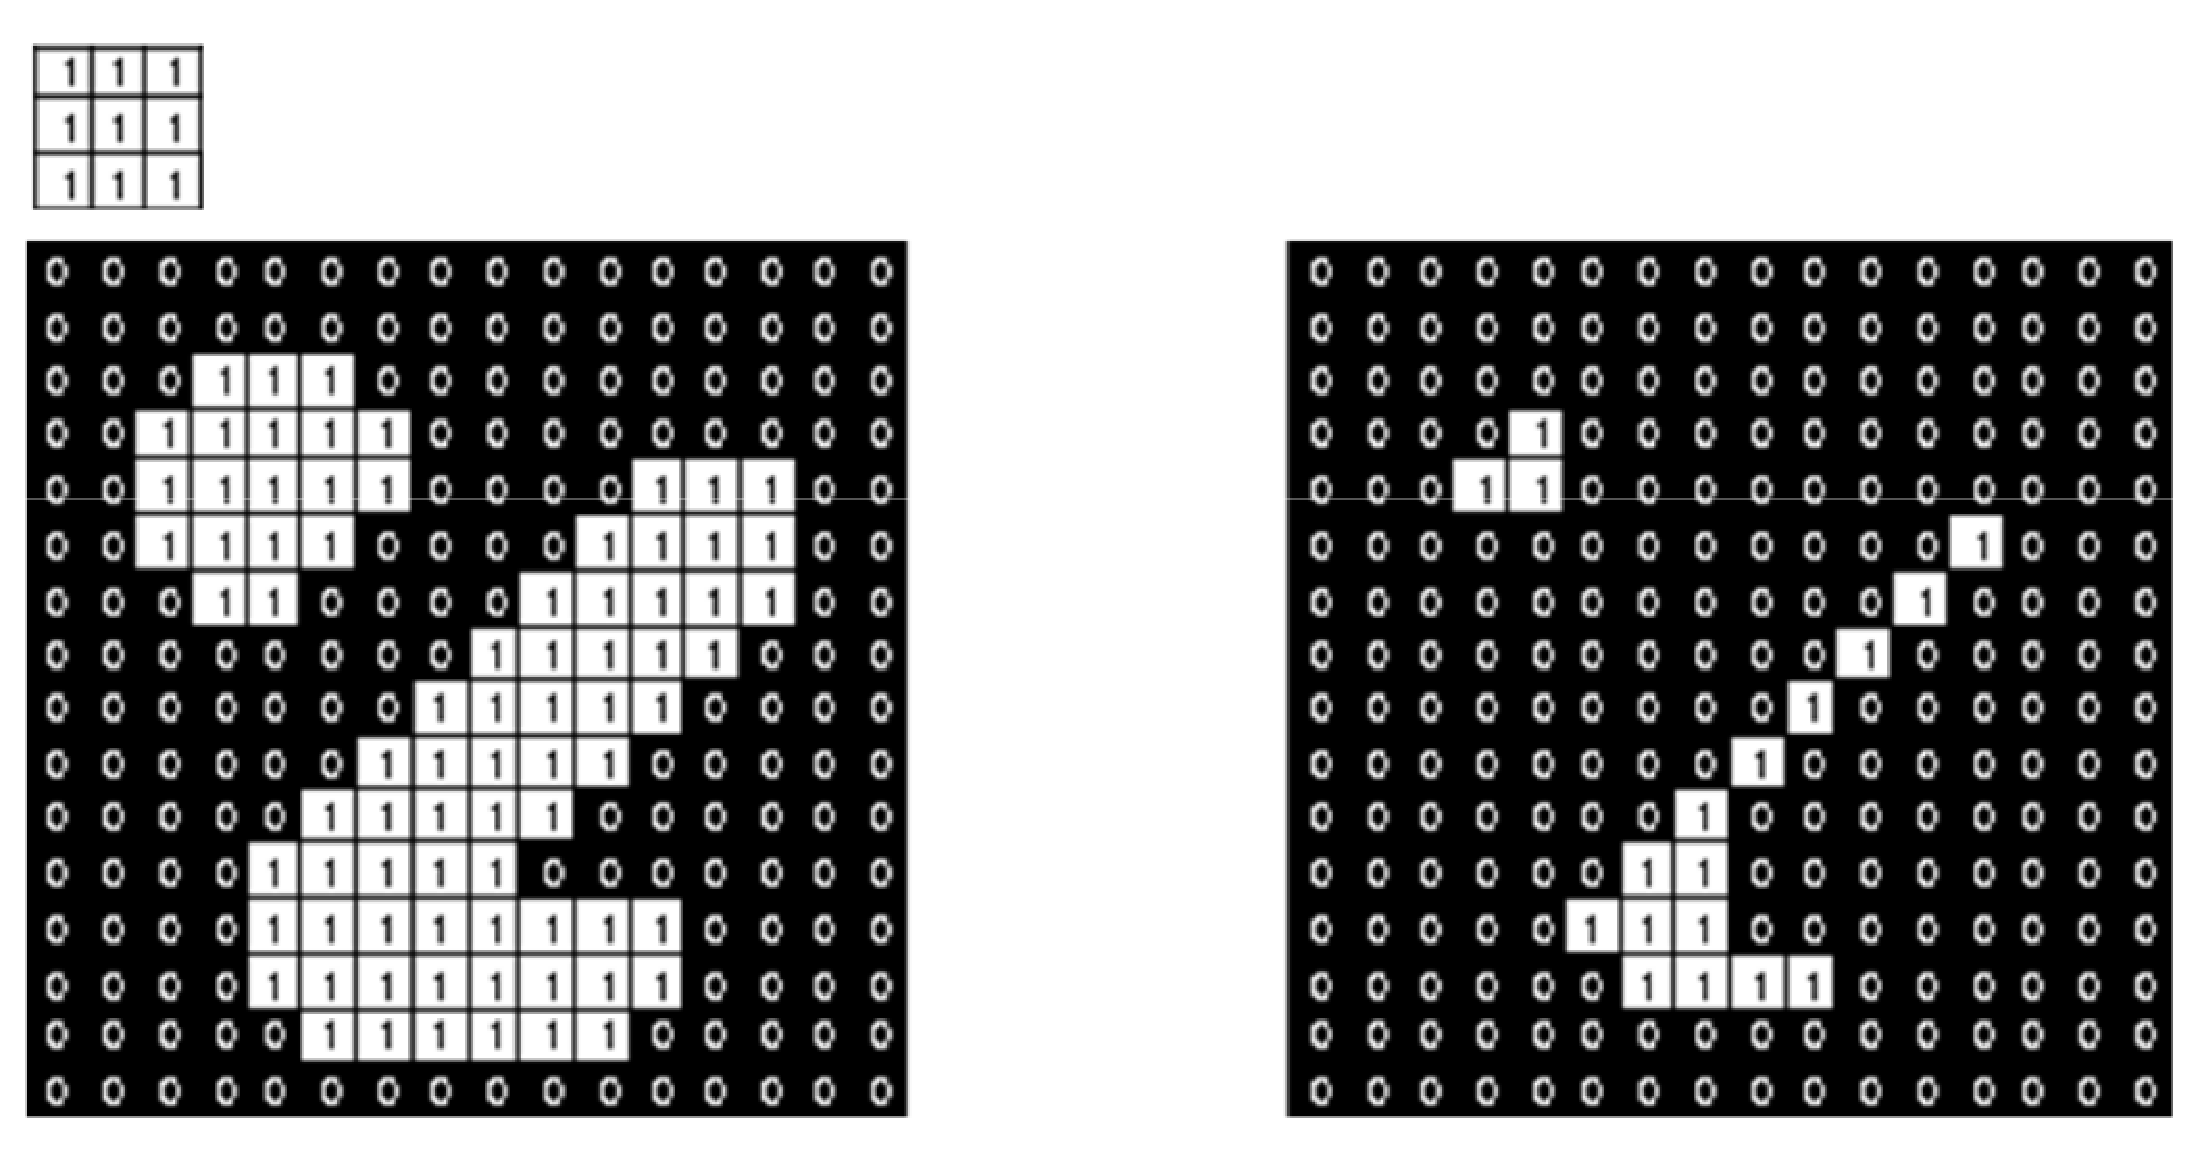
\includegraphics[width = 7.5 cm]{Erosao}
  \caption{Exemplo da opera\c{c}\~ao morfol\'ogica: Eros\~ao. \`A esquerda \'e a imagem original, \`a direita \'e a imagem erudida. Fonte: fornecido pelo professor.}
  \label{fig:erosao}
\end{figure}

\subsubsection{Dilata\c{c}\~ao}
A dilata\c{c}\~ao \'e definida como sendo:
$$ A \oplus B  = \{z \mid (\hat{B})_z \cap A \neq \emptyset \},$$
ou seja, a dilata\c{c}\~ao de $A$ por $B$ \'e o conjunto de todos os deslocamentos $z$ de forma que $B$ e $A$ se sobrep\~oem, em pelo menos, por um elemento, como demonstrado na Figura~\ref{fig:dilata}; um modo alternativo:
$$ A \oplus B  = \{z \mid [(\hat{B})_z \cap A] \subseteq A \}.$$

\begin{figure}[]
  \centering
  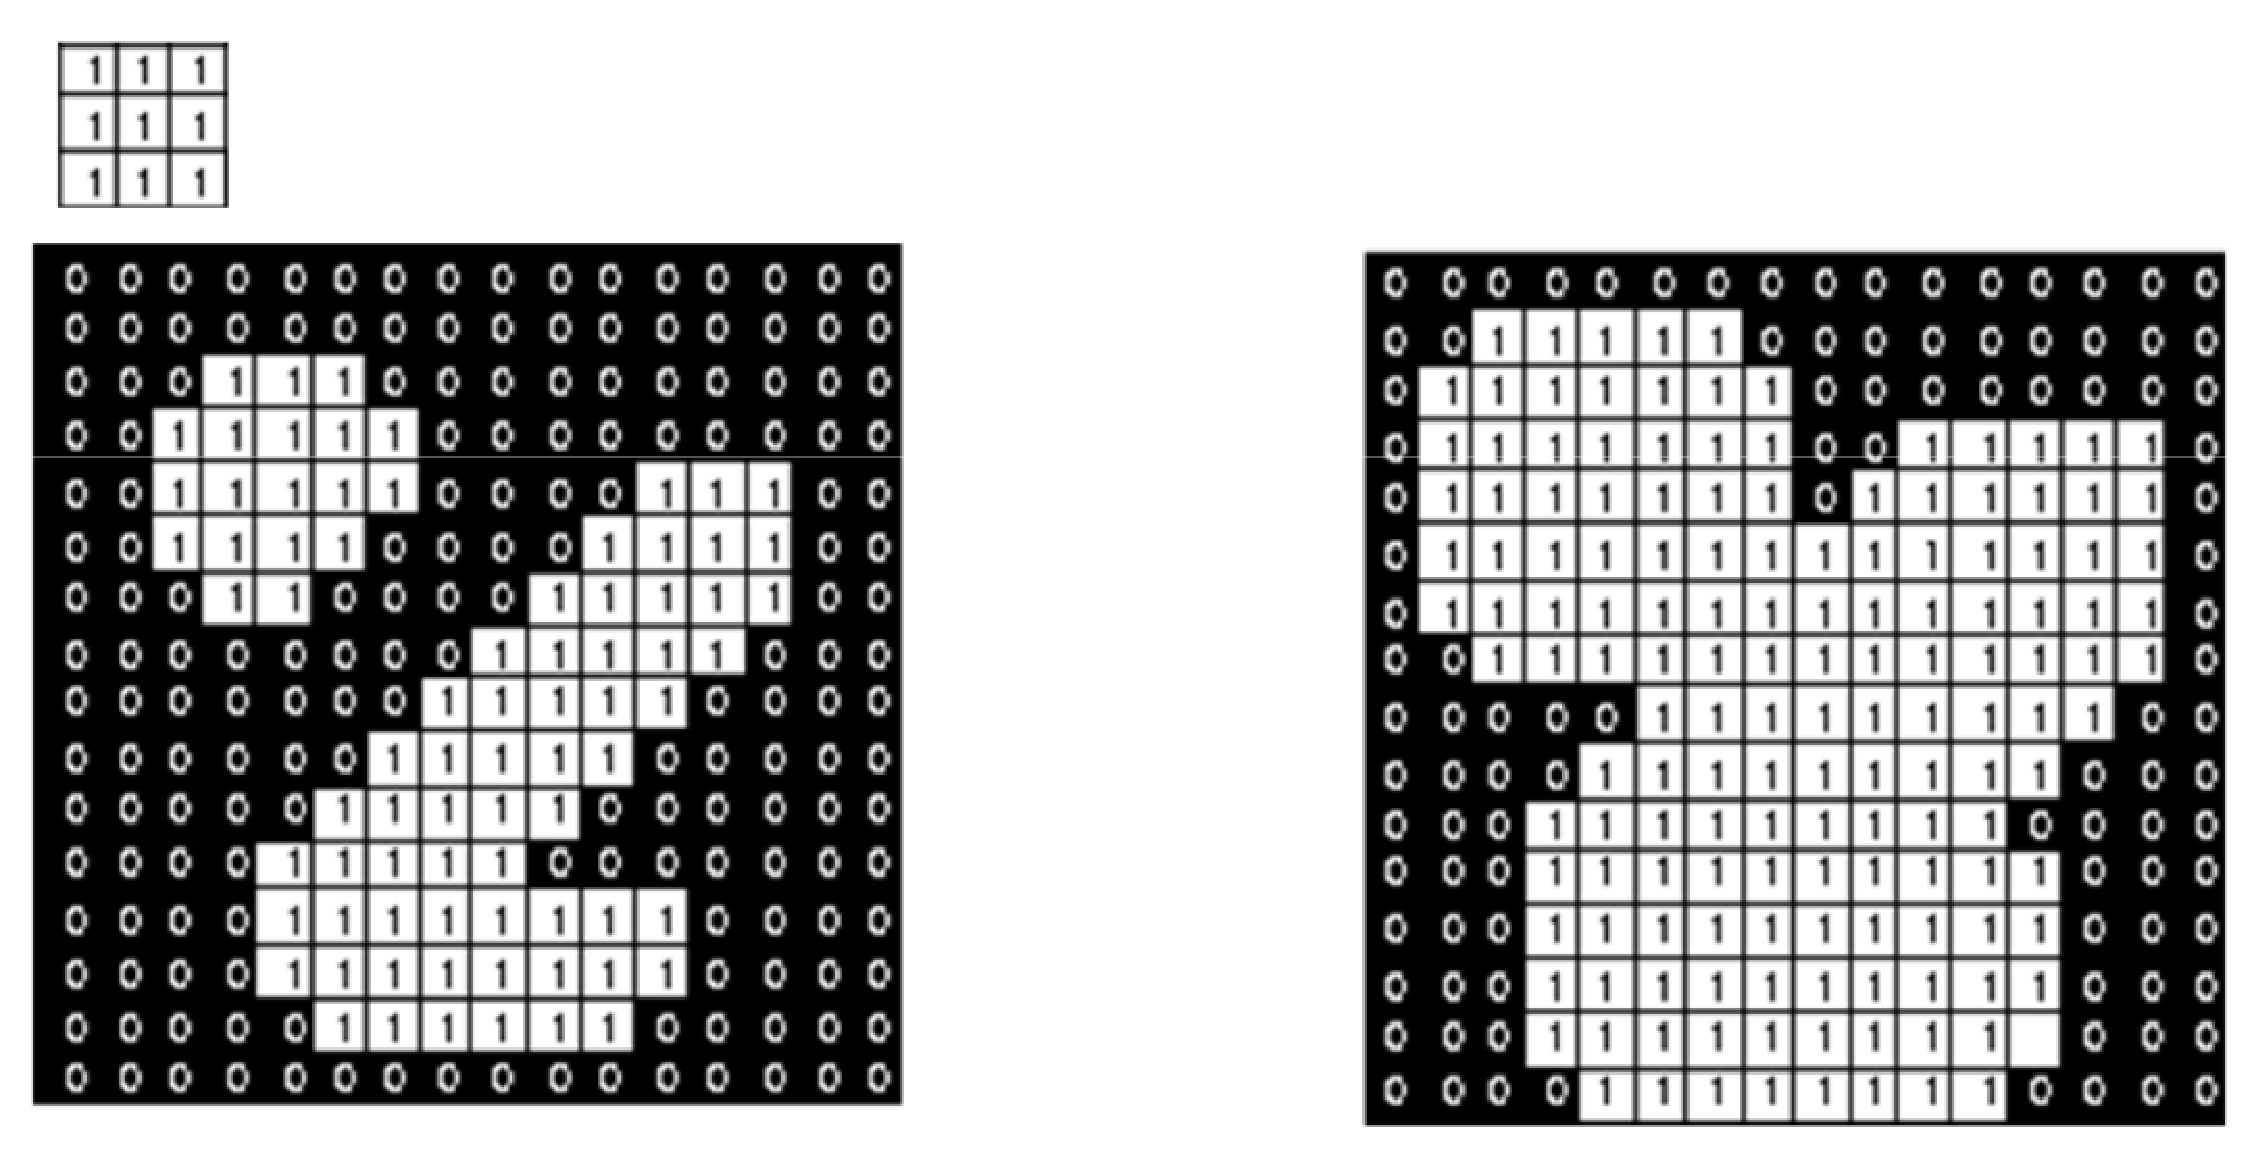
\includegraphics[width = 7.5 cm]{Dilatacao}
  \caption{Exemplo da opera\c{c}\~ao morfol\'ogica: Dilata\c{c}\~ao. \`A esquerda \'e a imagem original, \`a direita \'e a imagem dilatada. Fonte: fornecido pelo professor.}
  \label{fig:dilata}
\end{figure}

\subsubsection{Fechamento}
O fechamento visa suavisar contornos como, tamb\'em, funde as descontinuidades estreitas e alonga os golfos finos, elimina pequenos buracos e preenche lacunas num contorno, sendo definida como sendo:
$$ A \bullet B = [(A \oplus B) \ominus B],$$
ou seja, consiste na dilata\c{c}\~ao de $A$ por $B$, seguida da eros\~ao do resultado por $B$, como demonstrado na Figura~\ref{fig:fecha}.

\begin{figure}[]
  \centering
  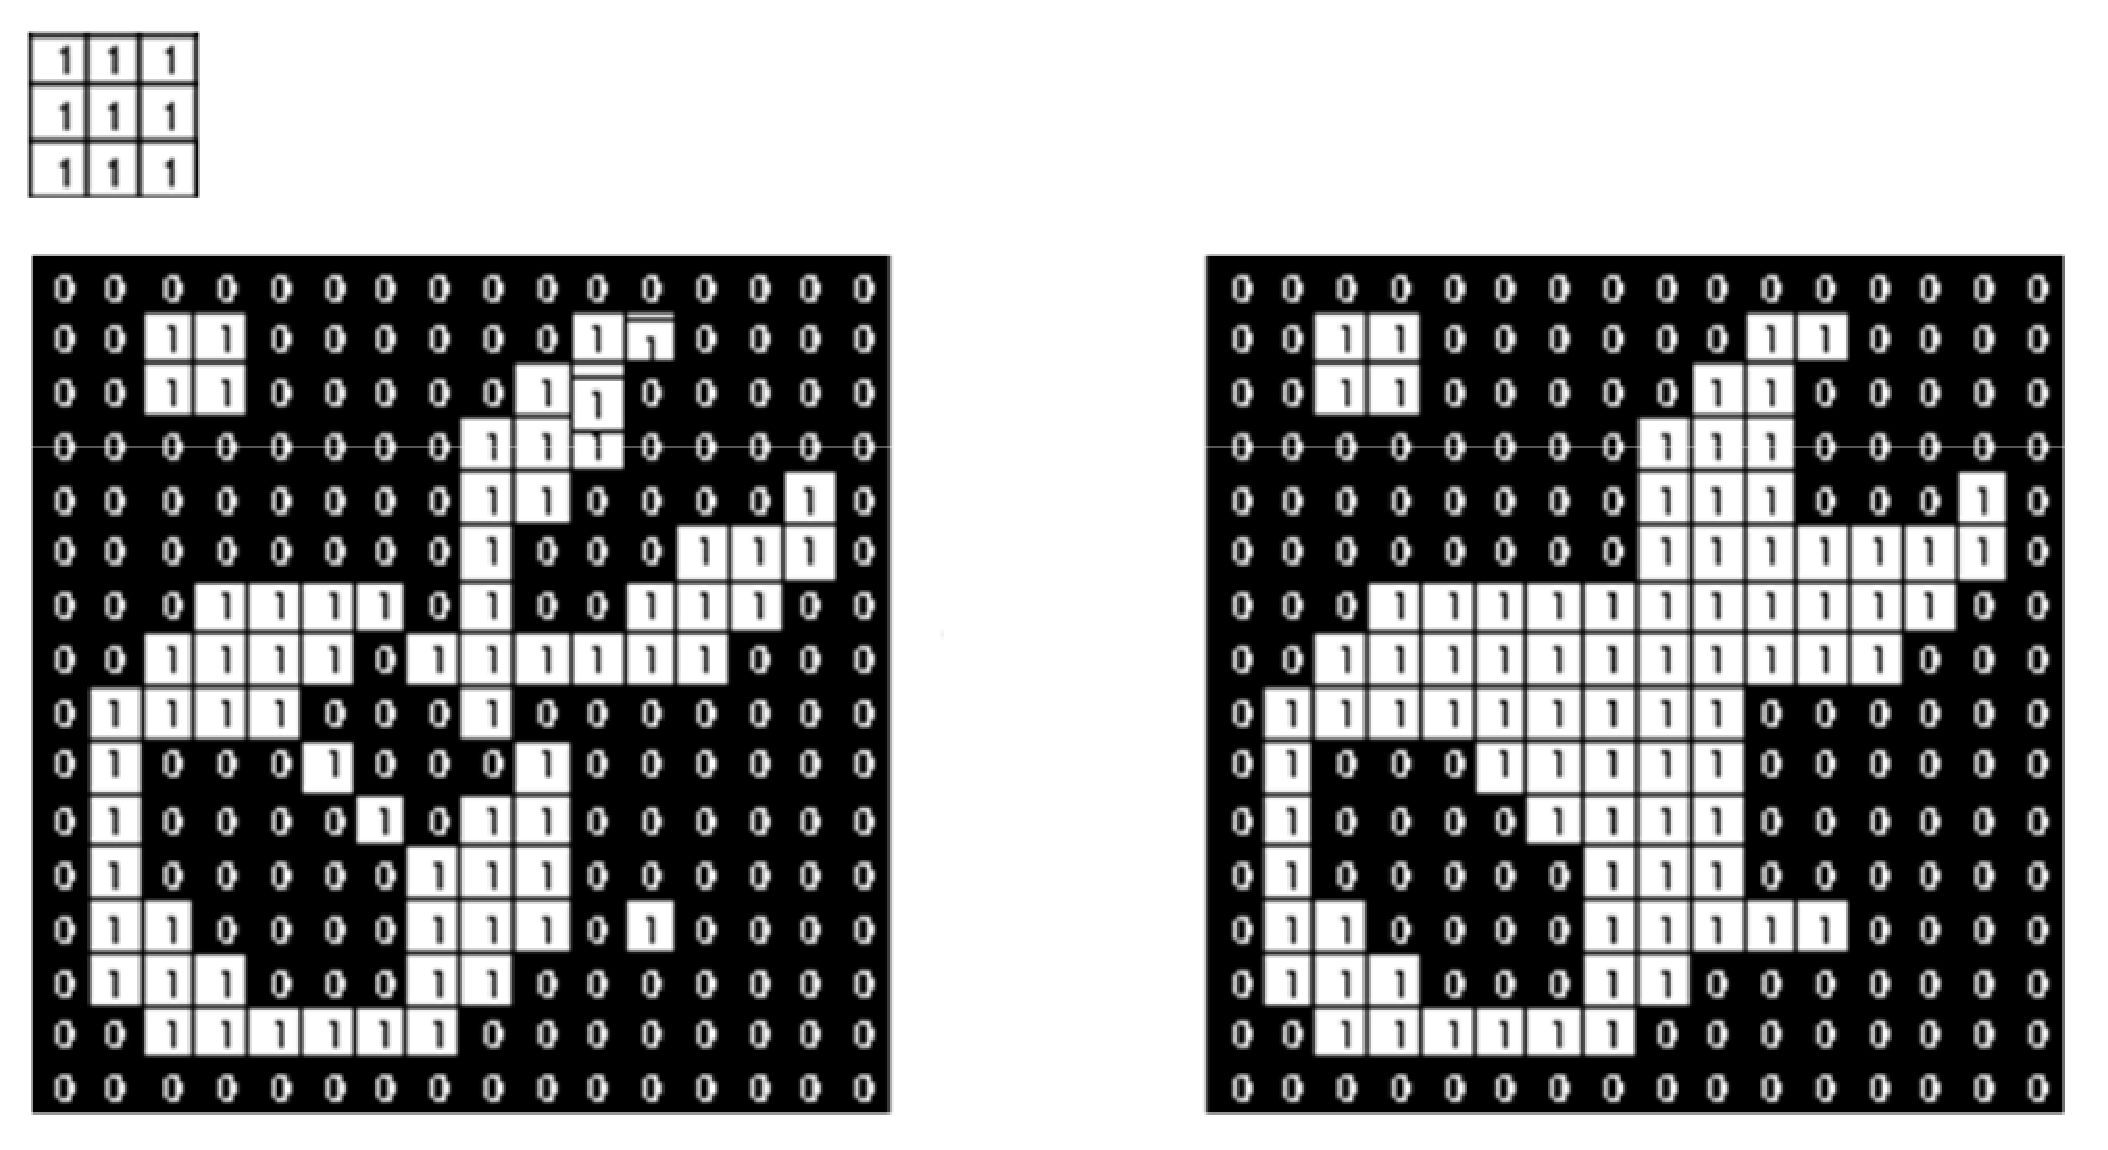
\includegraphics[width = 7.5 cm]{Fechamento}
  \caption{Exemplo da opera\c{c}\~ao morfol\'ogica: Fechamento. \`A esquerda \'e a imagem original, \`a direita \'e a imagem dilatada. Fonte: fornecido pelo professor.}
  \label{fig:fecha}
\end{figure}

\subsubsection{Top-Hat e Bottom-Hat}
A transformada~\textit{Top-Hat} \'e, normalmente, utilizada para real\c{c}\~ar objetos claros sobre um fundo escuro, enquanto que a~\textit{Bottom-Hat} \'e utilizada para real\c{c}ar objetos escuros sobre o fundo claro. Dessa forma, \'e comumente afirmado de que a transformada~\textit{Top-Hat} ajuda a ver detalhes em partes escuras da imagem; a~\textit{Bottom-Hat} ajuda a visualizar detalhes em partes claras.

A partir disso, ao considerar $f$ como a imagem original e $b$ como o elemento estruturante, tem-se as defini\c{c}\~oes como sendo:
$$ Top = f - (f \circ b),$$ 
$$ Bottom = (f \bullet b) - f.$$

\subsubsection{Watershed}
Segundo Alexandre~\cite{water} ``a transformada de~\textit{watershed} \'e um dos operadores cl\'assicos para segmenta\c{c}\~ao de imagens. Este operador simula a inunda\c{c}\~ao da superf\'icie de uma imagem cinza por fontes de \'aguas colocadas em~\textit{pixels} semelhantes; erguendo uma barreira toda vez que \'aguas provenientes de fontes distintas se encontram, impedindo, assim, que elas se misturem. As fontes s\~ao normalmente colocadas no fundo de bacias distintas da imagem.''


\section{Metodologia}
Com as defini\c{c}\~oes feitas \'e poss\'ivel prosseguir para o desenvolvimento do projeto. Dessa forma, esta se\c{c}\~ao visa apresentar os passos seguidos para a realiza\c{c}\~ao das atividades, desenvolvidas em ~\textbf{\textit{MatLab}}~\cite{matlab}. Como o projeto \'e constitu\'ido por tr\^es partes, estas ser\~ao abordadas separadamente.

\subsection{Circuito de Placa PCB}
Este problema espec\'ifico tem como base a Figura~\ref{fig:prob1.1} e visa contar a quantidade de buracos e determinar seus di\^ametros em~\textit{pixels}, visto que em sistemas autom\'aticos de inspe\c{c}\~ao de circuitos impressos \'e necess\'ario saber se \'e poss\'ivel inserir os componentes com ou sem dificuldades.

Foi realizado uma opera\c{c}\~ao de fechamento na imagem, pois havia buracos que n\~ao estavam totalmente isolados do restante da placa, seguida pela nega\c{c}\~ao dos valores dos pixels, de forma a preparar para futuras manipula\c{c}\~oes.

Com a imagem preenchida e negativada foi realizada a detec\c{c}\~ao das regi\~oesda imagem, sendo detectadas mais regi\~oes do que as de interesse, por isso foi realizado um refinamento sobre as regi\~oes, rejeitando as que n\~ao estivessem na faixa de tamanho esperado para as regi\~oes de interesse.

  \begin{figure}[]
    \centering
    
\includegraphics[width = 4.5 cm]{pcb}
    \caption{Imagem base, problema $1$. Fonte: fornecido pelo professor.}
    \label{fig:prob1.1}
  \end{figure}
%  ~
%  \begin{figure}[]
%    \centering
%    
\includegraphics[width = 3.5 cm]{Imagem_Binarizada_negativo}
%    \caption{Resultado da opera\c{c}\~ao morfol\'ogica, Fechamento, al\'em de negativa\c{c}\~ao dos~\textit{pixels}, problema $1$.}
%    \label{fig:prob1.2}
%  \end{figure}
%  ~
%  \begin{figure}[]
%    \centering
%    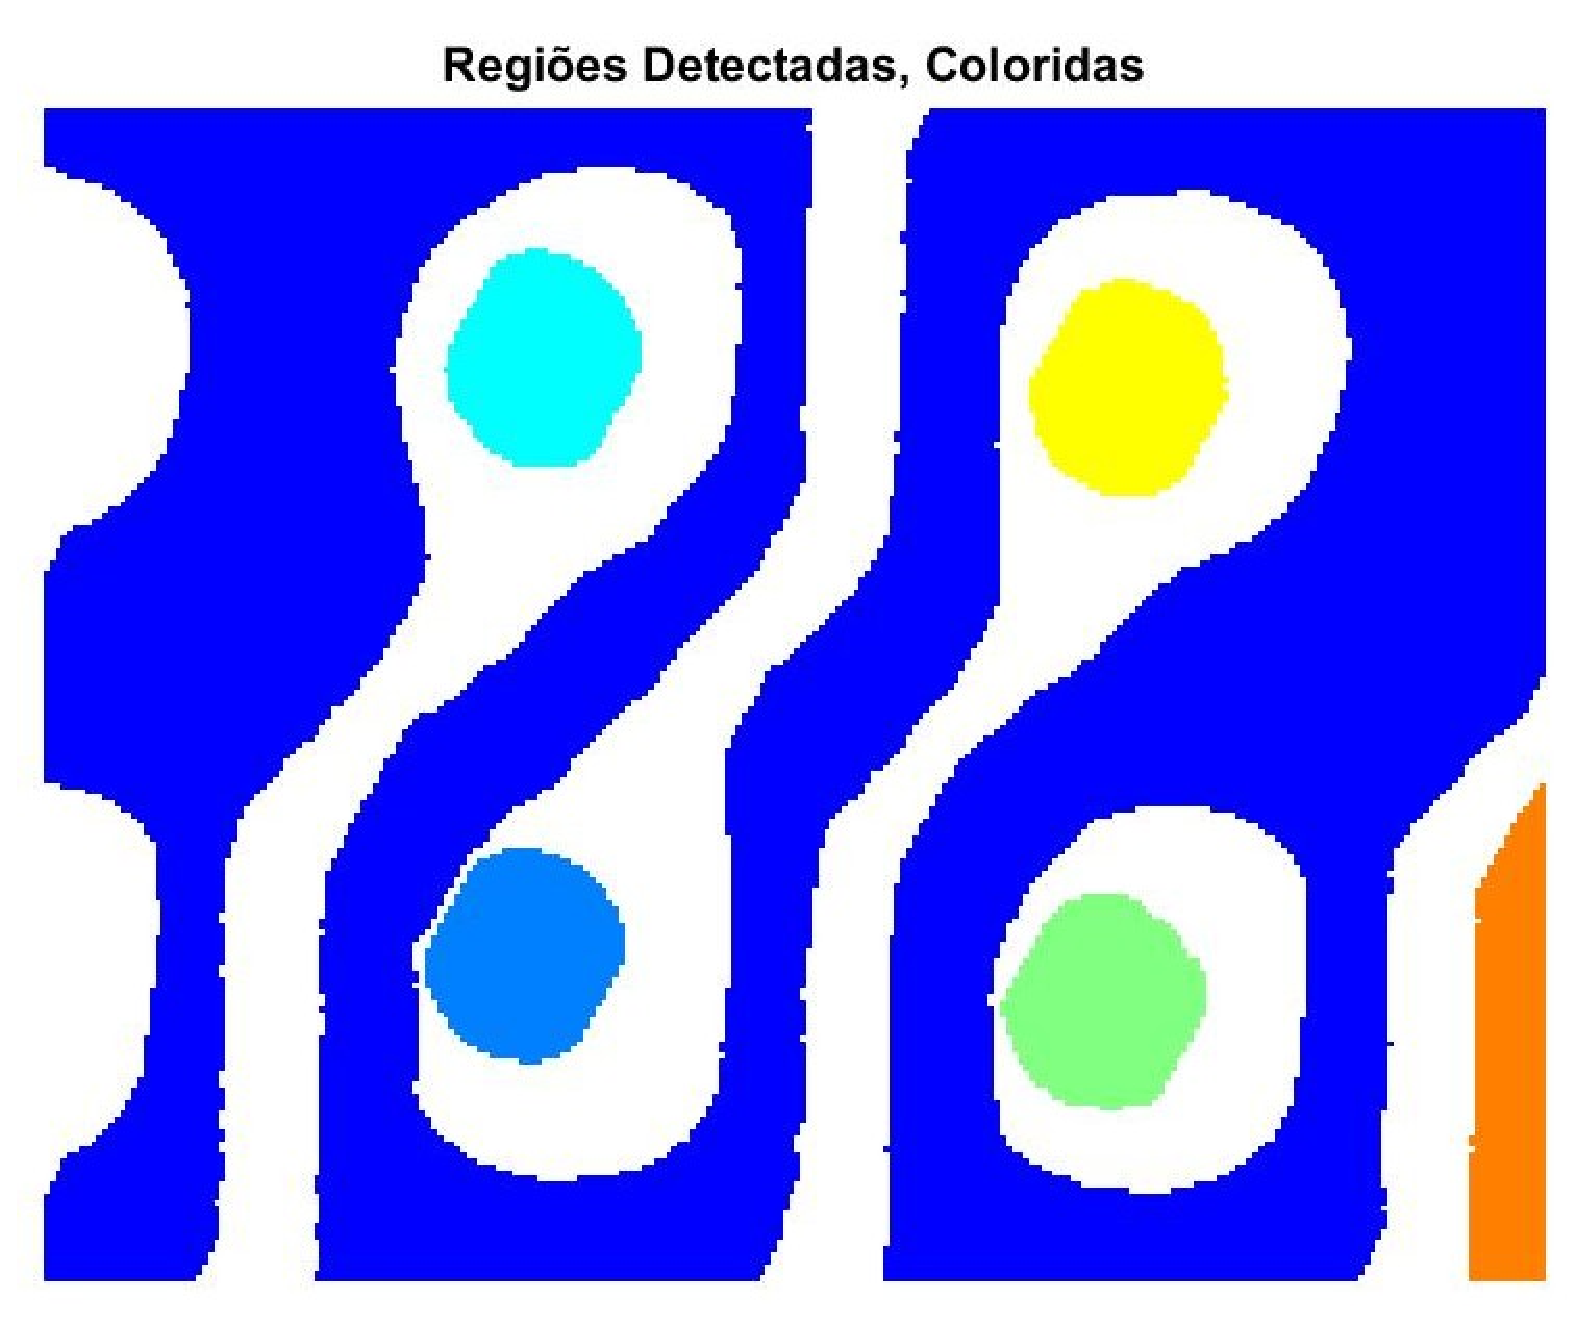
\includegraphics[width = 3.5 cm]{Regi_es_Detectadas_Coloridas_}
%    \caption{Resultado da determina\c{c}\~ao das regi\~oes da Figura~\ref{fig:prob1.2}, problema $1$.}
%    \label{fig:prob1.3}
%  \end{figure}


\subsection{Texto sobre Imagem}
Este problema espec\'ifico tem como base a Figura~\ref{fig:prob2.1} e visa retornar uma imagem bin\'aria de fundo branco e texto preto.

Foi implementado um pr\'e-processamento na imagem, por ter certo ru\'ido na imagem, para isso foi utilizado um filtro passa-baixa, o de m\'edia, amenizando tal inc\^omodo.

Foram empregadas as opera\c{c}\~oes morfol\'ogicas:~\textit{Top-Hat} e~\textit{Bottom-Hat}, para que pudesse ser ressaltado o fundo e o texto, respectivamente. A partir das imagens geradas anteriormente, foi realiza uma binariza\c{c}\~ao sobre cada uma, com limiares diferentes, com o intuito de tornar o texto preto e o fundo branco.

Ap\'os isso, foi realizado um realce do~\textit{background} da imagem atrav\'es da opera\c{c}\~ao morfol\'ogica fechamento, resultando numa imagem de puro~\textit{background}. Logo em seguida, foi retirado a imagem original da imagem resultado da opera\c{c}\~ao anterior, de forma a destacar o texto do fundo preto. 

\begin{figure}[!t]
  \centering
  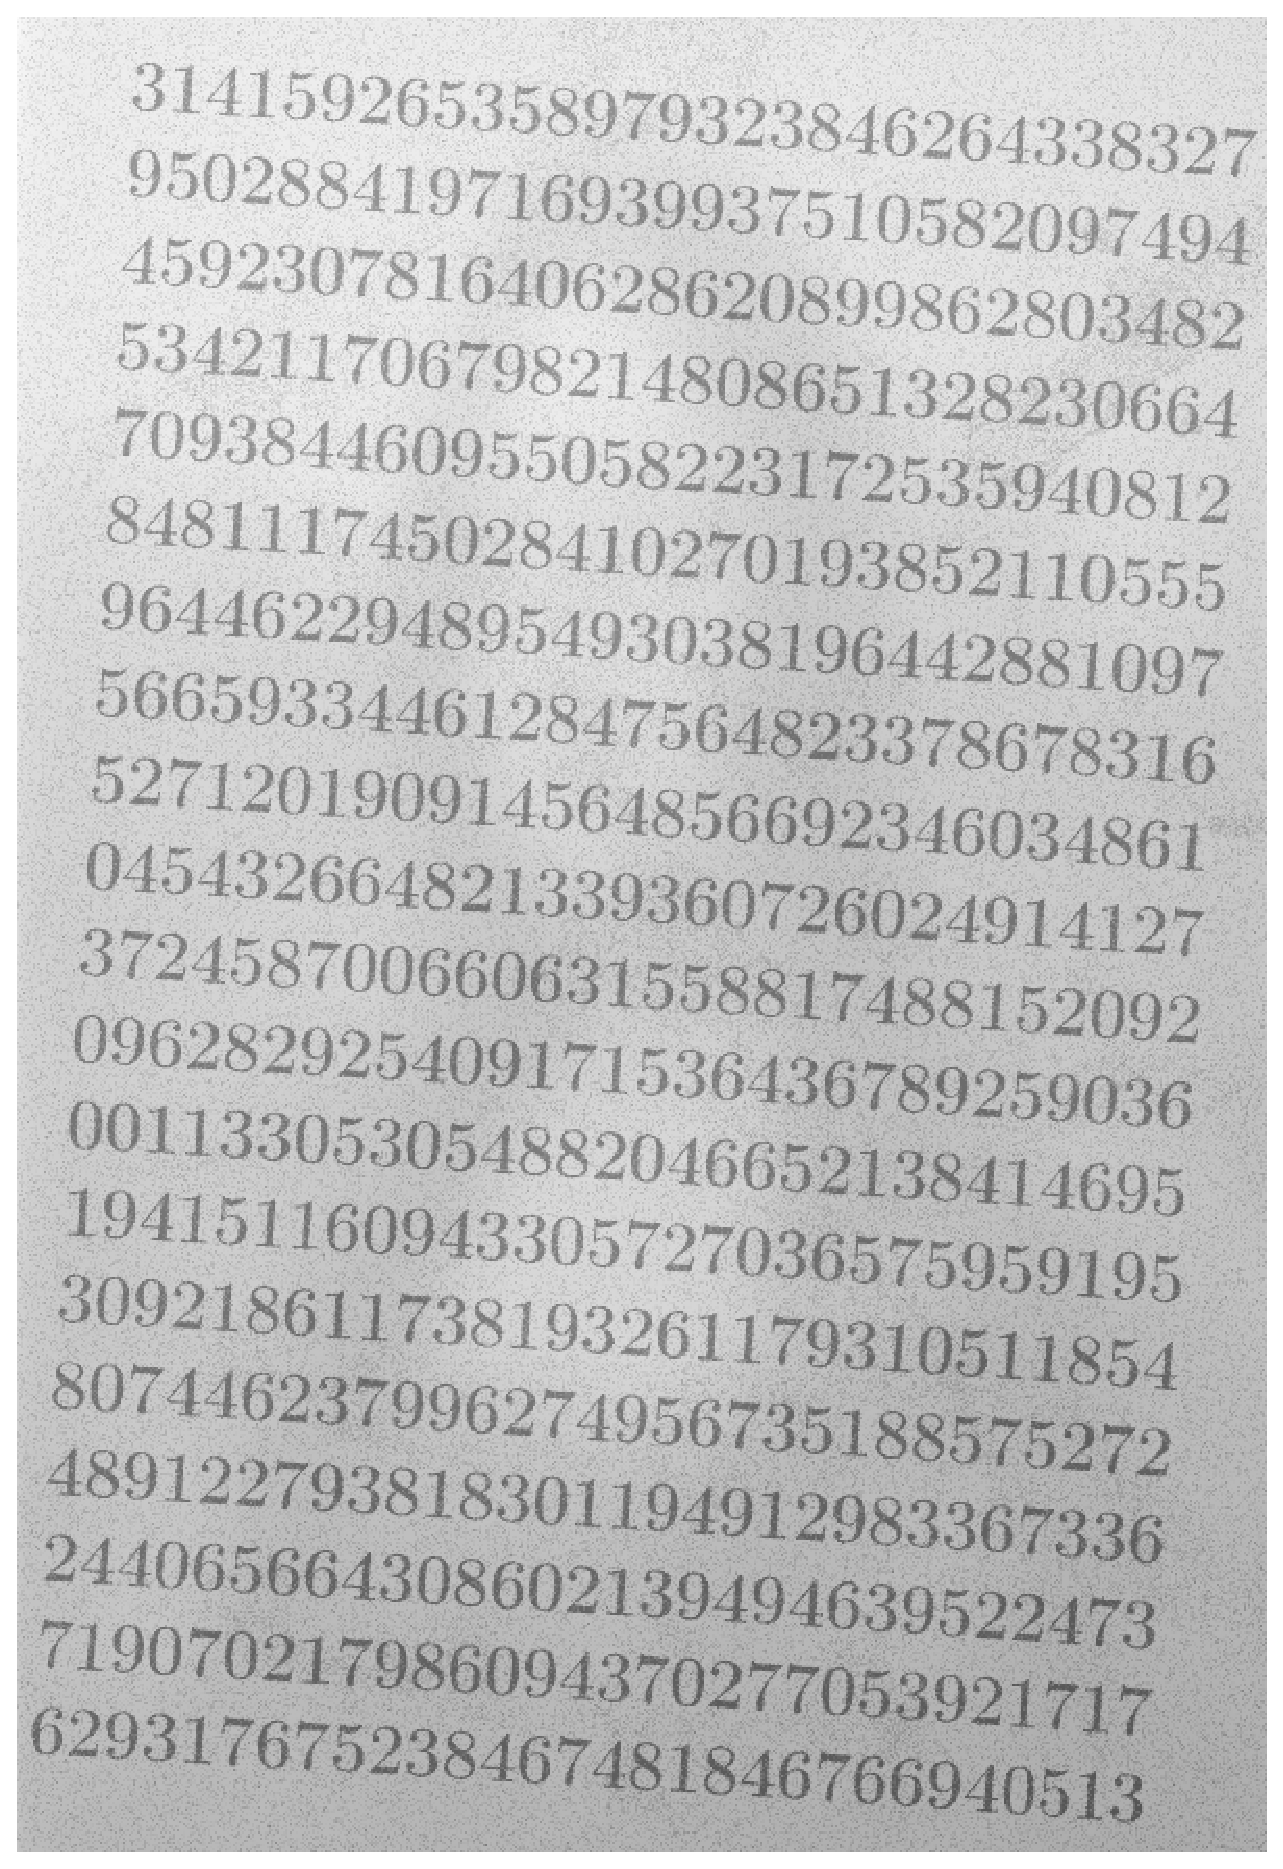
\includegraphics[width = 4.5 cm]{morf_test}
  \caption{Imagem base, problema $2$. Fonte: fornecido pelo professor.}
  \label{fig:prob2.1}
\end{figure}

\subsection{C\'elulas}
Este problema espec\'ifico tem como base a Figura~\ref{fig:prob3.1} e visa retornar uma imagem de fundo branco e as c\'elulas pretas.

Foi implementado um pr\'e-processamento na imagem, por ter certo ru\'ido na imagem, para isso foi utilizado um filtro passa-baixa, o de m\'edia, amenizando tal inc\^omodo. Em seguida, foi realizada a binariza\c{c}\~ao da imagem, considerando $145$ como~\textit{thershold}, seguida pela opera\c{c}\~ao negativa\c{c}\~ao da imagem resultado, com a finalidade de se obter c\'elulas brancas e fundo preto. Para a maioria das c\'elulas binarizadas foi observado a exist\^encia de buracos , por isso foi realizado a opera\c{c}\~ao de preenchimento de tais buracos.

Visando a determina\c{c}\~ao da dist\^ancia dos~\textit{pixels} at\'e os centr\'oides das regi\~oes foram consideradas as imagem binaria preenchida e sua negativa, uma imagem de dist\^ancia foi gerada para cada uma.

Logo ap\'os foi implementado a opera\c{c}\~ao morfol\'ogica de~\textit{Watershed}, a fim de obter as regi\~oes por profundidade.

\begin{figure}[!t]
  \centering
  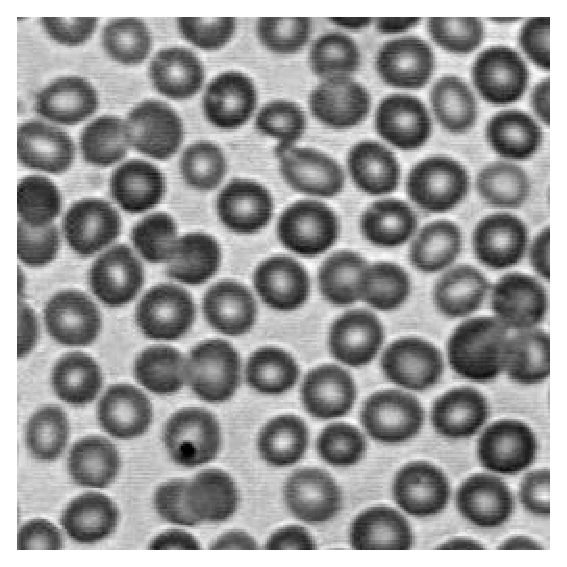
\includegraphics[width = 4.5 cm]{img_cells}
  \caption{Imagem base, problema $3$. Fonte: fornecido pelo professor.}
  \label{fig:prob3.1}
\end{figure}



\section{Resultados}
Como dito na se\c{c}\~ao ``Metodologia'' h\'a tr\^es problemas, dessa forma esta se\c{c}\~ao tamb\'em ser\'a subdividida sobre tais problemas como segue. Todos os c\'odigos est\~ao dispon\'iveis~\textit{online}~\cite{down}, assim como todas as imagens-resultado obtidas com a execu\c{c}\~ao dos~\textit{scripts}.

\subsection{Circuito de Placa PCB}
Seguindo os passos determinados na metodologia, obteve-se a Figura~\ref{fig:prob1.2} como resultado da opera\c{c}\~ao morfol\'ogica de fechamento seguida pela negativa\c{c}\~ao dos valores dos~\textit{pixels}.

Foram detectadas as regi\~oes da imagem, como demonstrado na Figura~\ref{fig:prob1.3}, a partir dela foi realizada o refinamento de tais regi\~oes, obtendo como resultado a Figura~\ref{fig:prob1.4}.

\begin{figure}[!t]
  \centering
  
\includegraphics[width = 4.5 cm]{Imagem_Binarizada_negativo}
  \caption{Imagem do circuito, ap\'os o fechamento e nega\c{c}\~ao.}
  \label{fig:prob1.2}
\end{figure}

\begin{figure}[!t]
  \centering
  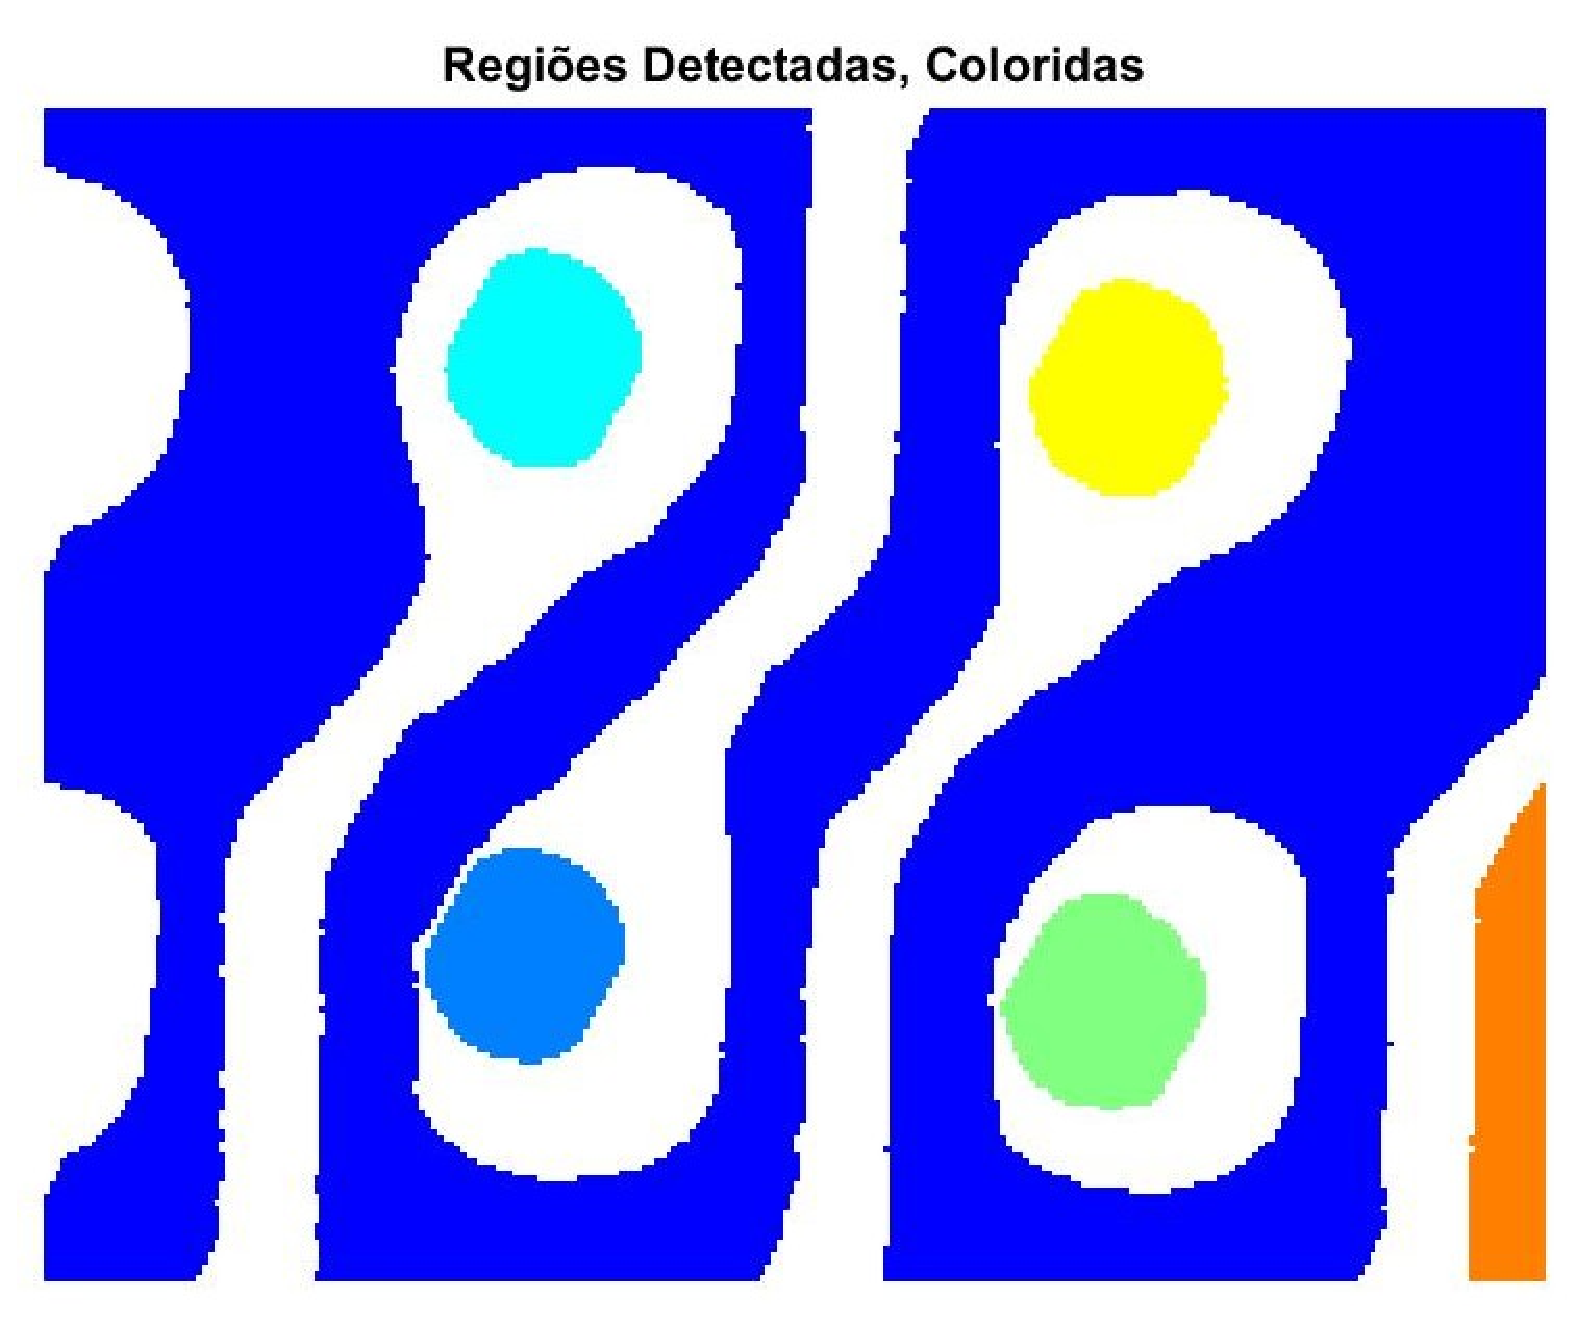
\includegraphics[width = 4.5 cm]{Regi_es_Detectadas_Coloridas_}
  \caption{Imagem do circuito, ap\'os a detec\c{c}\~ao das regi\~oes.}
  \label{fig:prob1.3}
\end{figure}

\begin{figure}[!t]
  \centering
  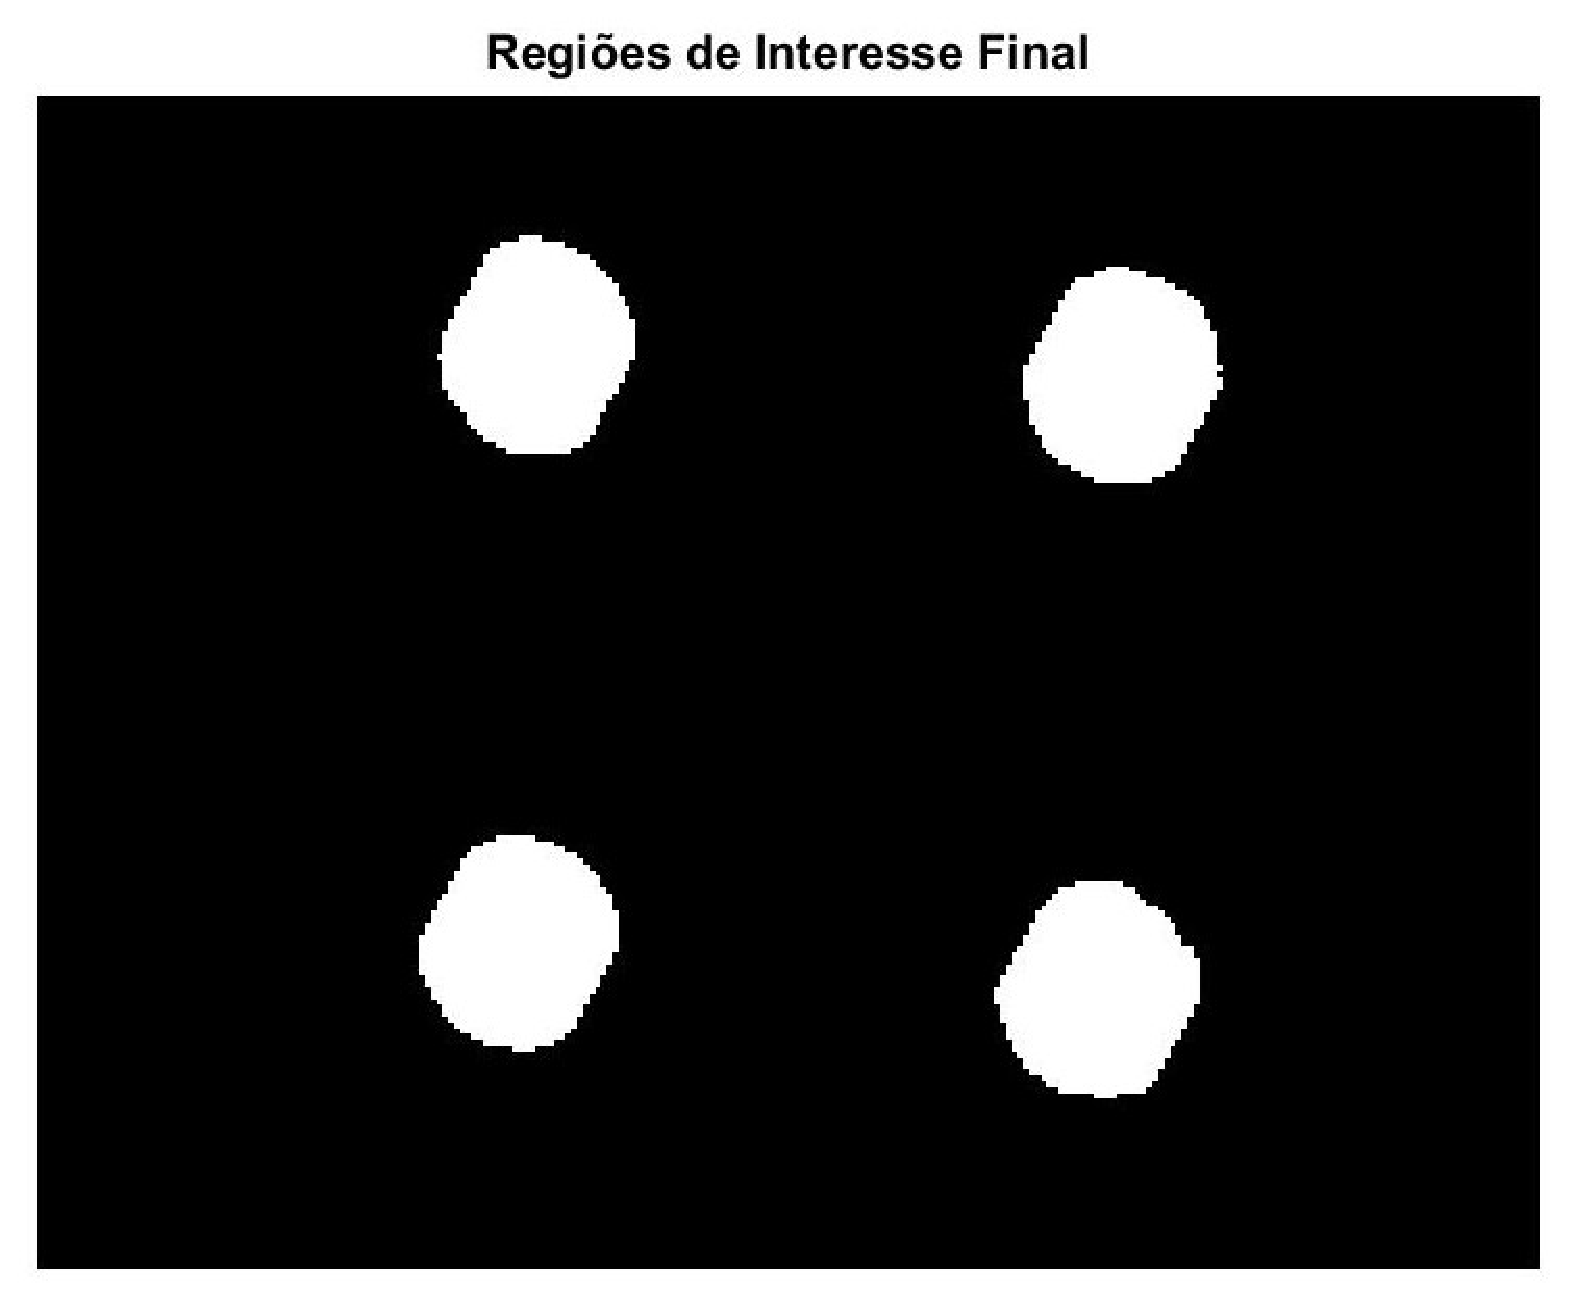
\includegraphics[width = 4.5 cm]{Regi_es_de_Interesse_Final_}
  \caption{Imagem do circuito, apenas as regi\~oes de interesse.}
  \label{fig:prob1.4}
\end{figure}

Dessa forma, foram detectadas quatro regi\~oes, consideradas de interesse, e para elas foram obtidos tais caracter\'isticas:~\textbf{1\textdegree Regi\~ao} com \'area de $933$~\textit{pixels} e di\^ametro m\'inimo de $34$~\textit{pixels};~\textbf{2\textdegree Regi\~ao} com \'area de $926$~\textit{pixels} e di\^ametro m\'inimo de $34$~\textit{pixels}; ~\textbf{3\textdegree Regi\~ao} com \'area de $951$~\textit{pixels} e di\^ametro m\'inimo de $35$~\textit{pixels} e a ~\textbf{4\textdegree Regi\~ao} com \'area de $943$~\textit{pixels} e di\^ametro m\'inimo de $34$~\textit{pixels}.



\subsection{Texto sobre Imagem}
Seguindo os passos determinados na metodologia, foram obtidas as Figuras~\ref{fig:prob2.2}~e~\ref{fig:prob2.3}, demonstrando as opera\c{c}~oes morfol\'ogicas~\textit{Top-Hat} e~\textit{Bottom-Hat}, respectivamente, sobre a imagem original de tal problema. A partir de cada uma delas, foi realizado uma opera\c{c}\~ao de binariza\c{c}\~ao da imagem, afim de se obter uma imagem de fundo branco e texto preto.

Al\'em disso, foi realizado um realce do~\textit{background}, por interm\'edio da opera\c{c}\~ao morfol\'ogica de fechamento., obtendo como resultado a Figura~\ref{fig:prob2.4}. A partir dela, foi realizada a subtra\c{c}\~ao da imagem original da mesma, obtendo uma imagem com apenas os n\'umeros.

\begin{figure}[!t]
  \centering
  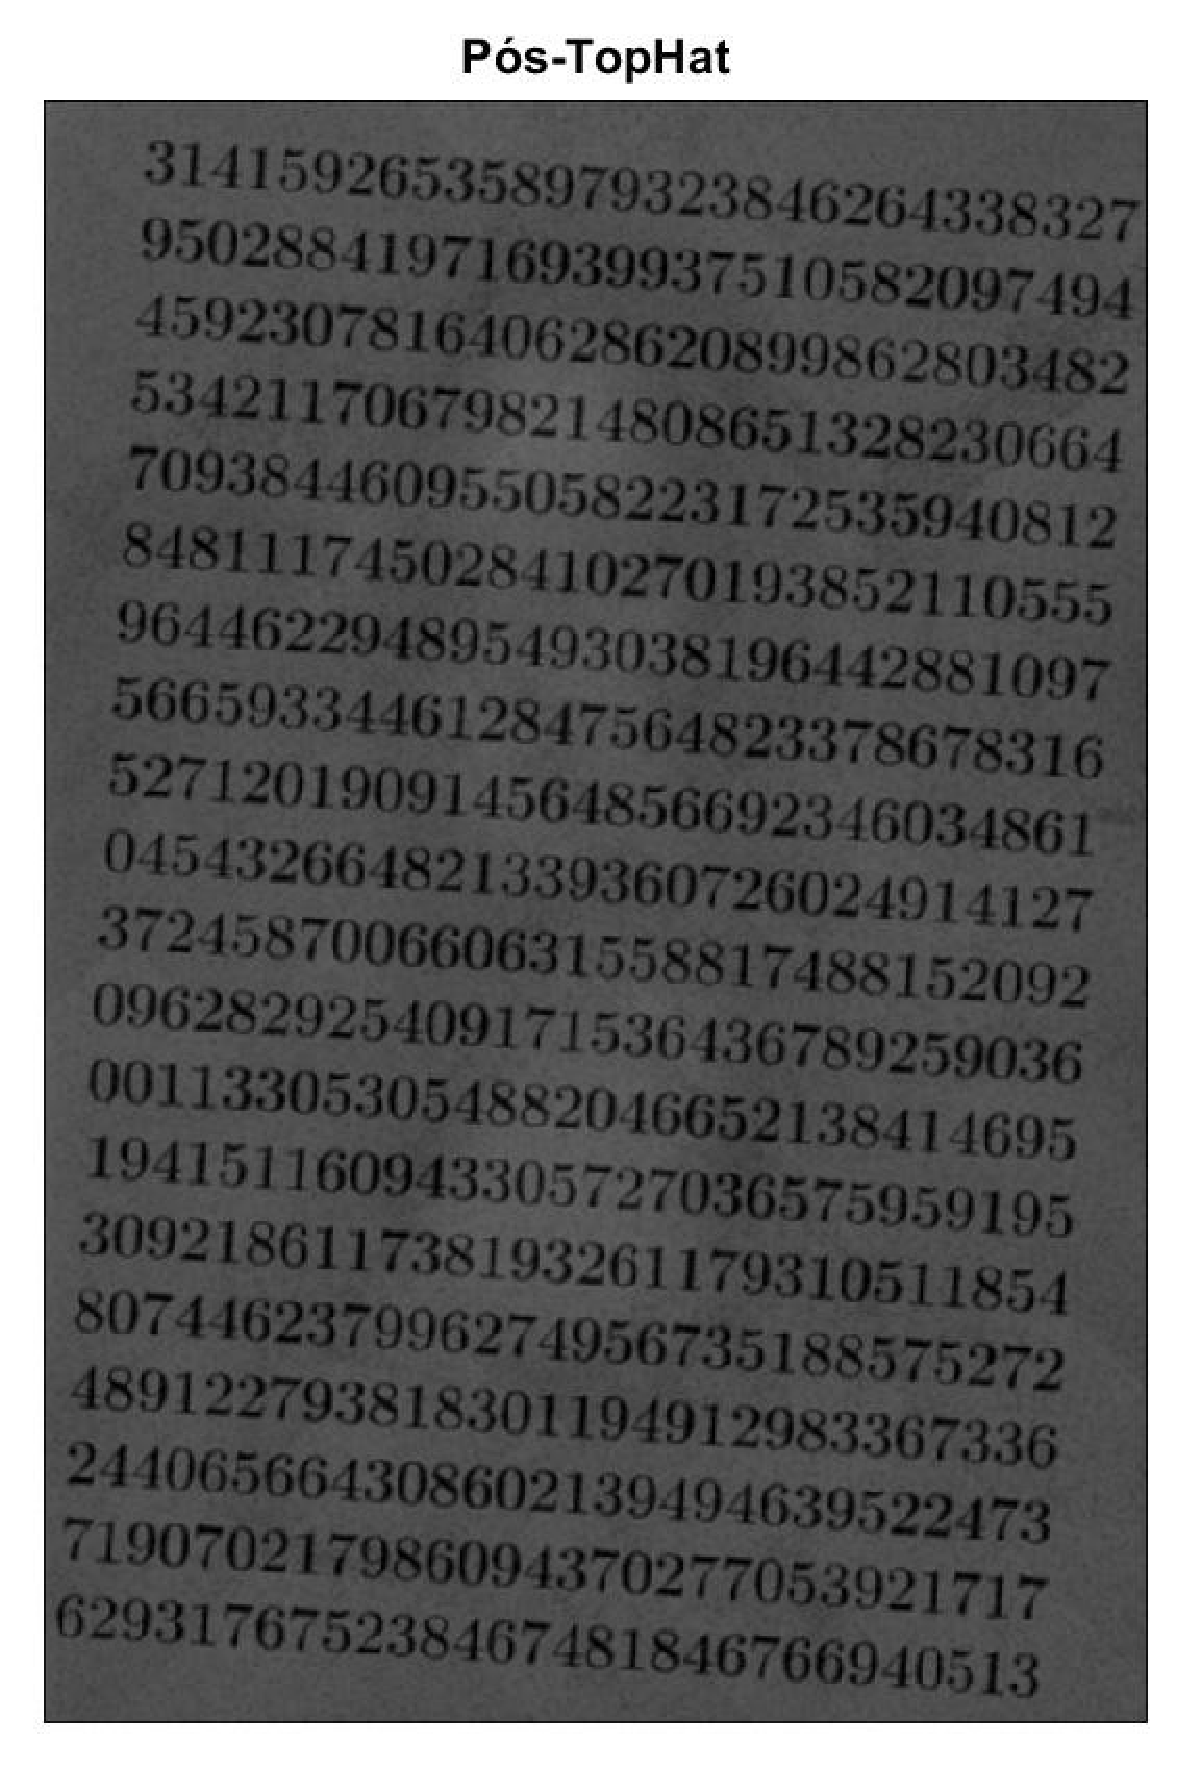
\includegraphics[width = 4.5 cm]{P_s-TopHat_}
  \caption{Imagem do texto sobre imagem, ap\'os a opera\c{c}\~ao Top-Hat.}
  \label{fig:prob2.2}
\end{figure}

\begin{figure}[!t]
  \centering
  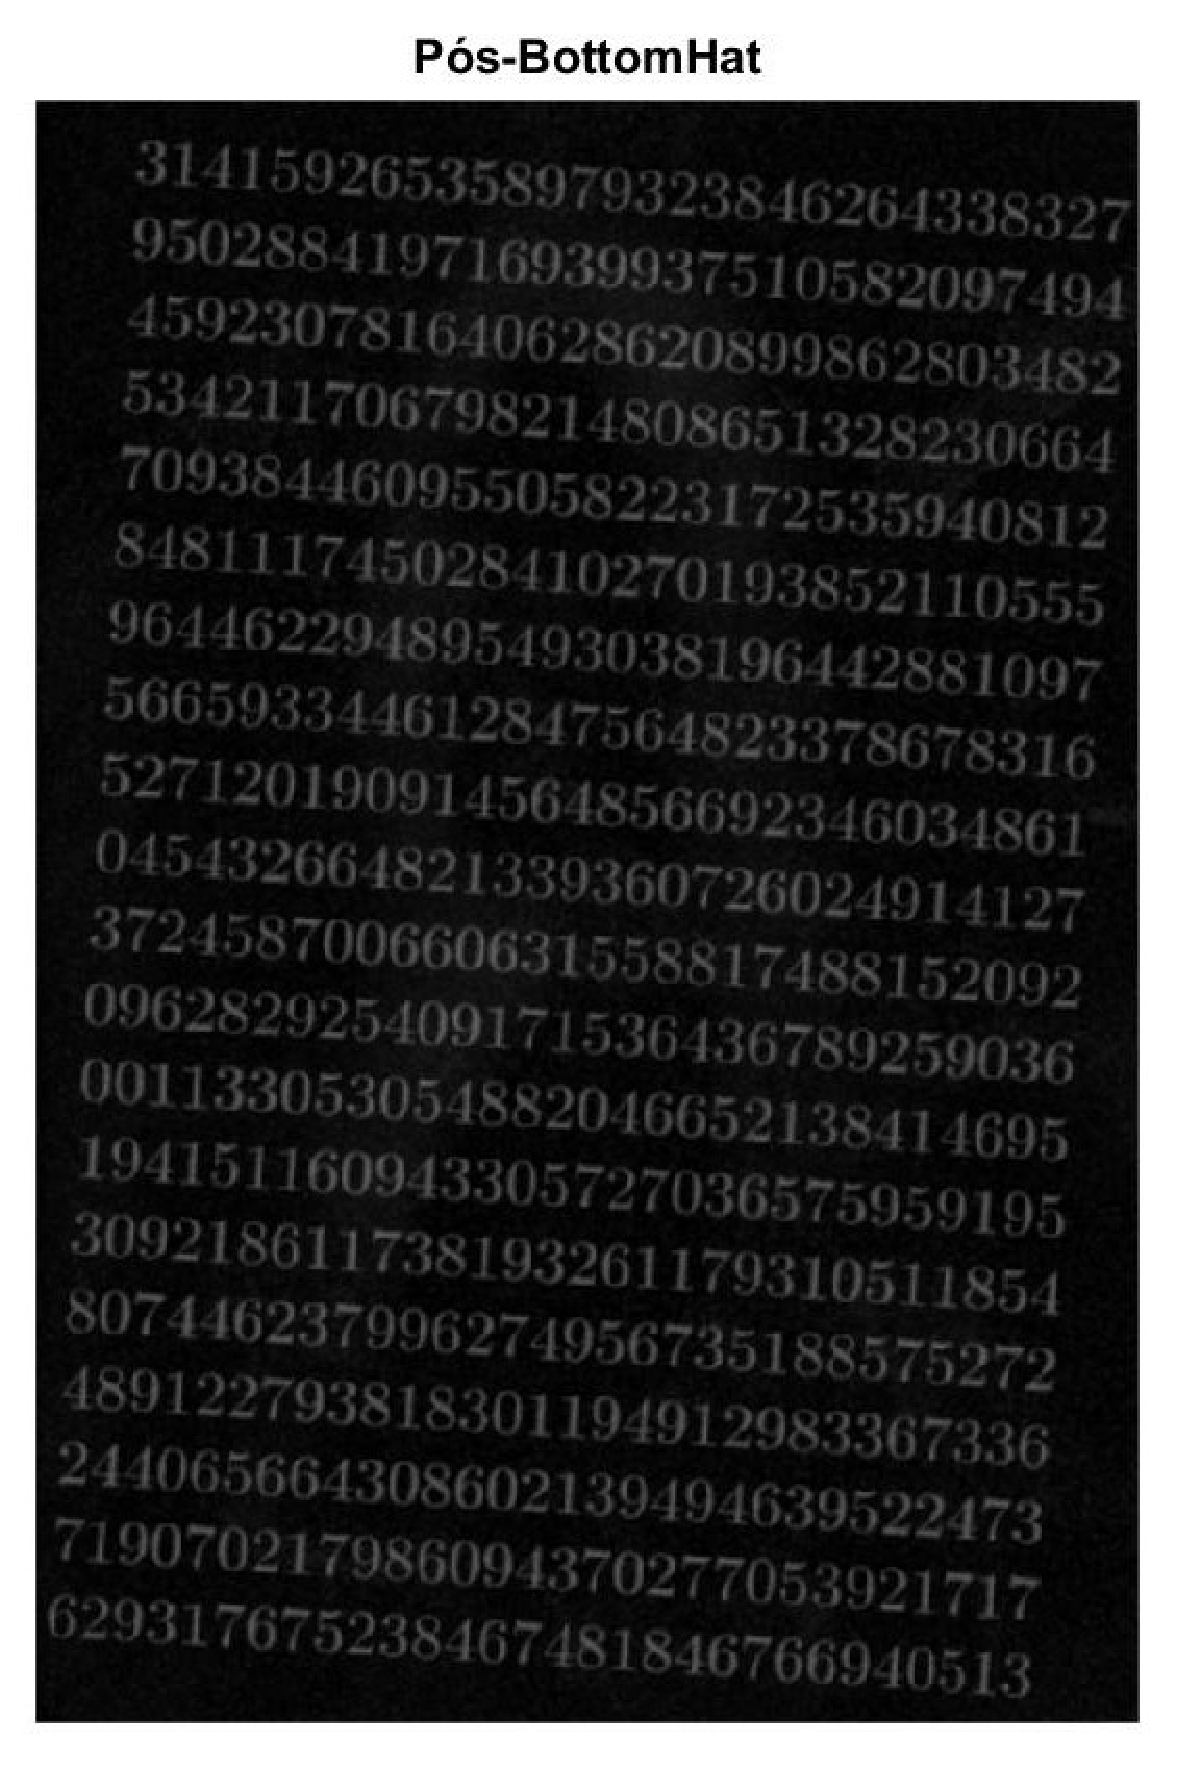
\includegraphics[width = 4.5 cm]{P_s-BottomHat_}
  \caption{Imagem do texto sobre imagem, ap\'os a opera\c{c}\~ao Bottom-Hat.}
  \label{fig:prob2.3}
\end{figure}

\begin{figure}[!t]
  \centering
  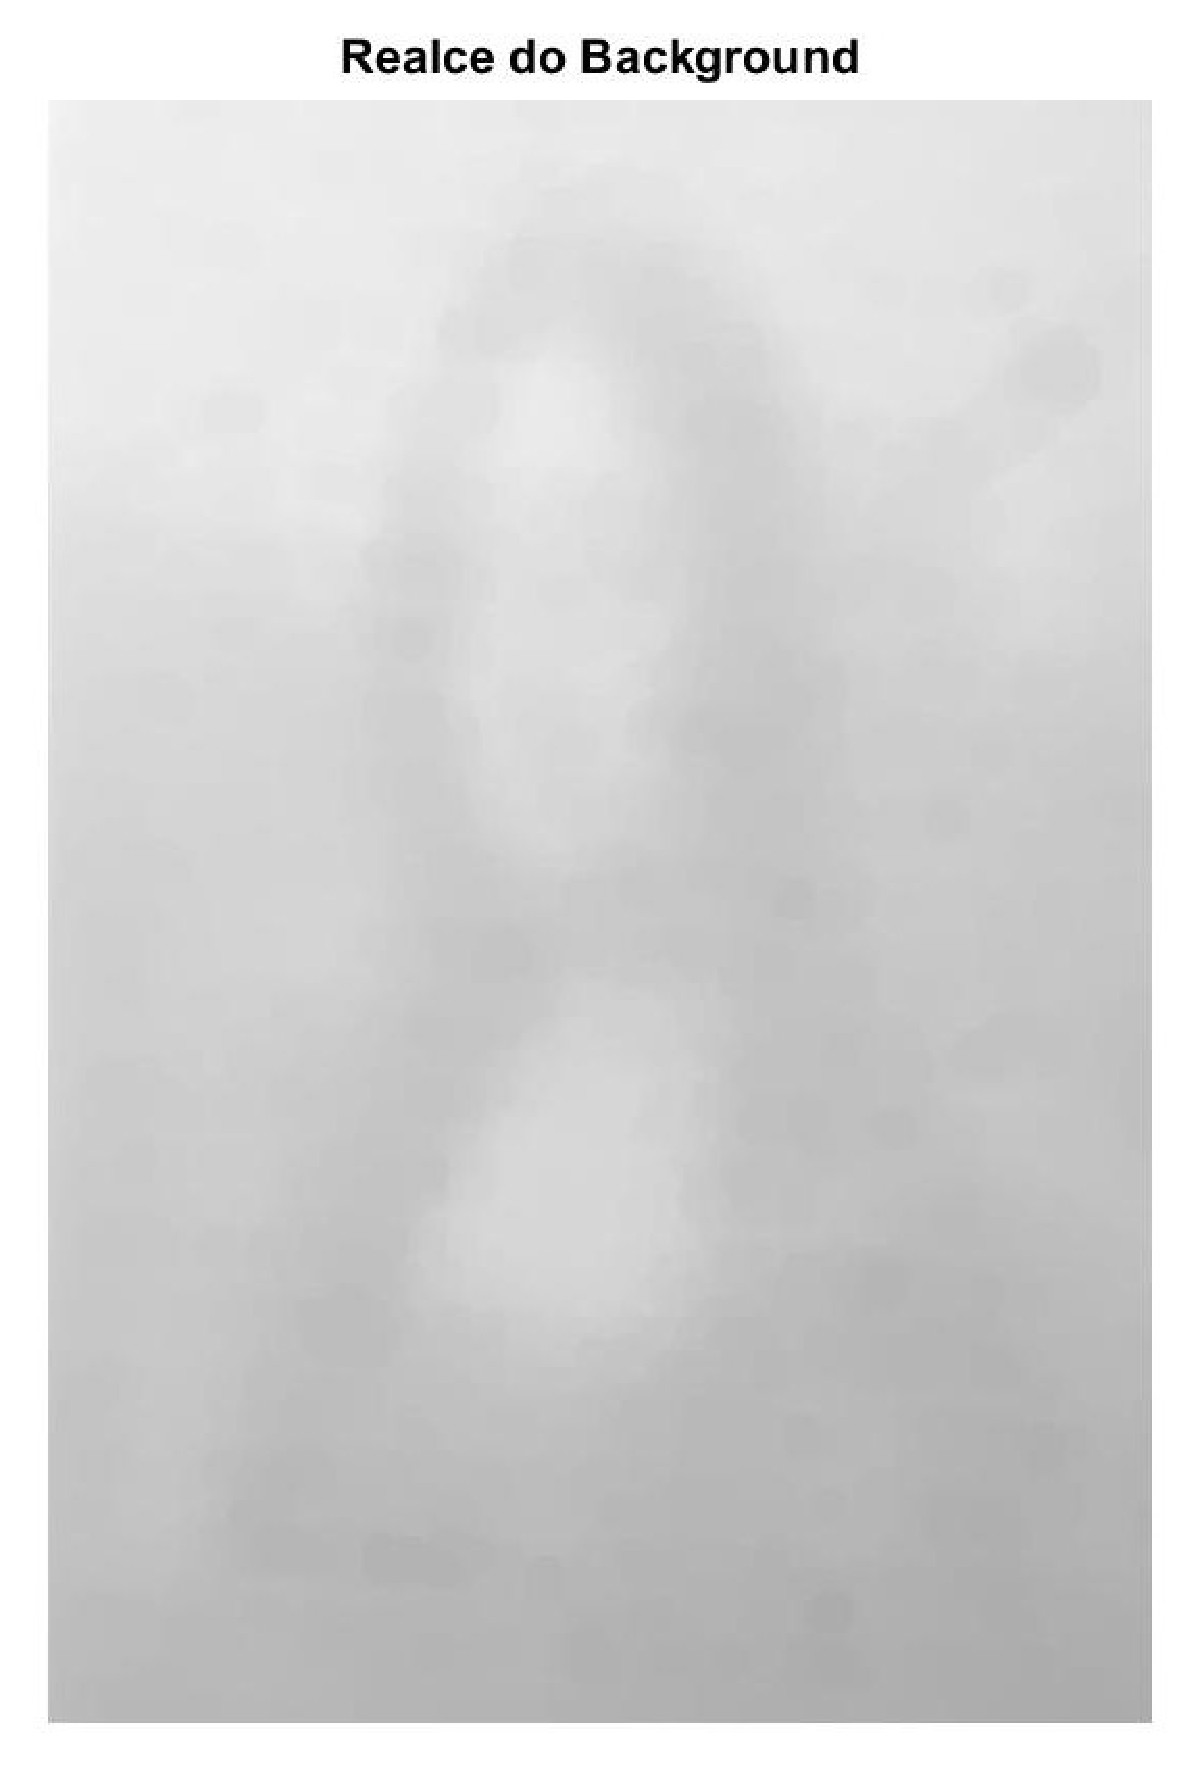
\includegraphics[width = 4.5 cm]{Realce_do_Background}
  \caption{Imagem do texto sobre imagem, ap\'os a opera\c{c}\~ao de Realce do Background.}
  \label{fig:prob2.4}
\end{figure}



\subsection{C\'elulas}
Seguindo os passos determinados na metodologia, foi obtida a Figura~\ref{fig:prob3.2}, que demonstra o resultado da binariza\c{c}\~ao seguida pelo preenchimento dos eventuais buracos.

A fim de determinar as dist\^ancias dos~\textit{pixels} at\'e os centr\'oides foi utilizado o negativo da Figura~\ref{fig:prob3.2}. Ao aplicar tal resultado sobre a imagem base obteve-se a Figura~\ref{fig:prob3.3}, como resultado. Utilizando esta mesma imagem, a opera\c{c}\~ao morfol\'ogica~\textit{Watershed} foi realizada e tem como resultado a Figura~\ref{fig:prob3.4}.

Como explicitado, h\'a, tamb\'em, a imagem das c\'elulas pretas e fundo branco, demonstrado na Figura~\ref{fig:prob3.5}.

\begin{figure}[!t]
  \centering
  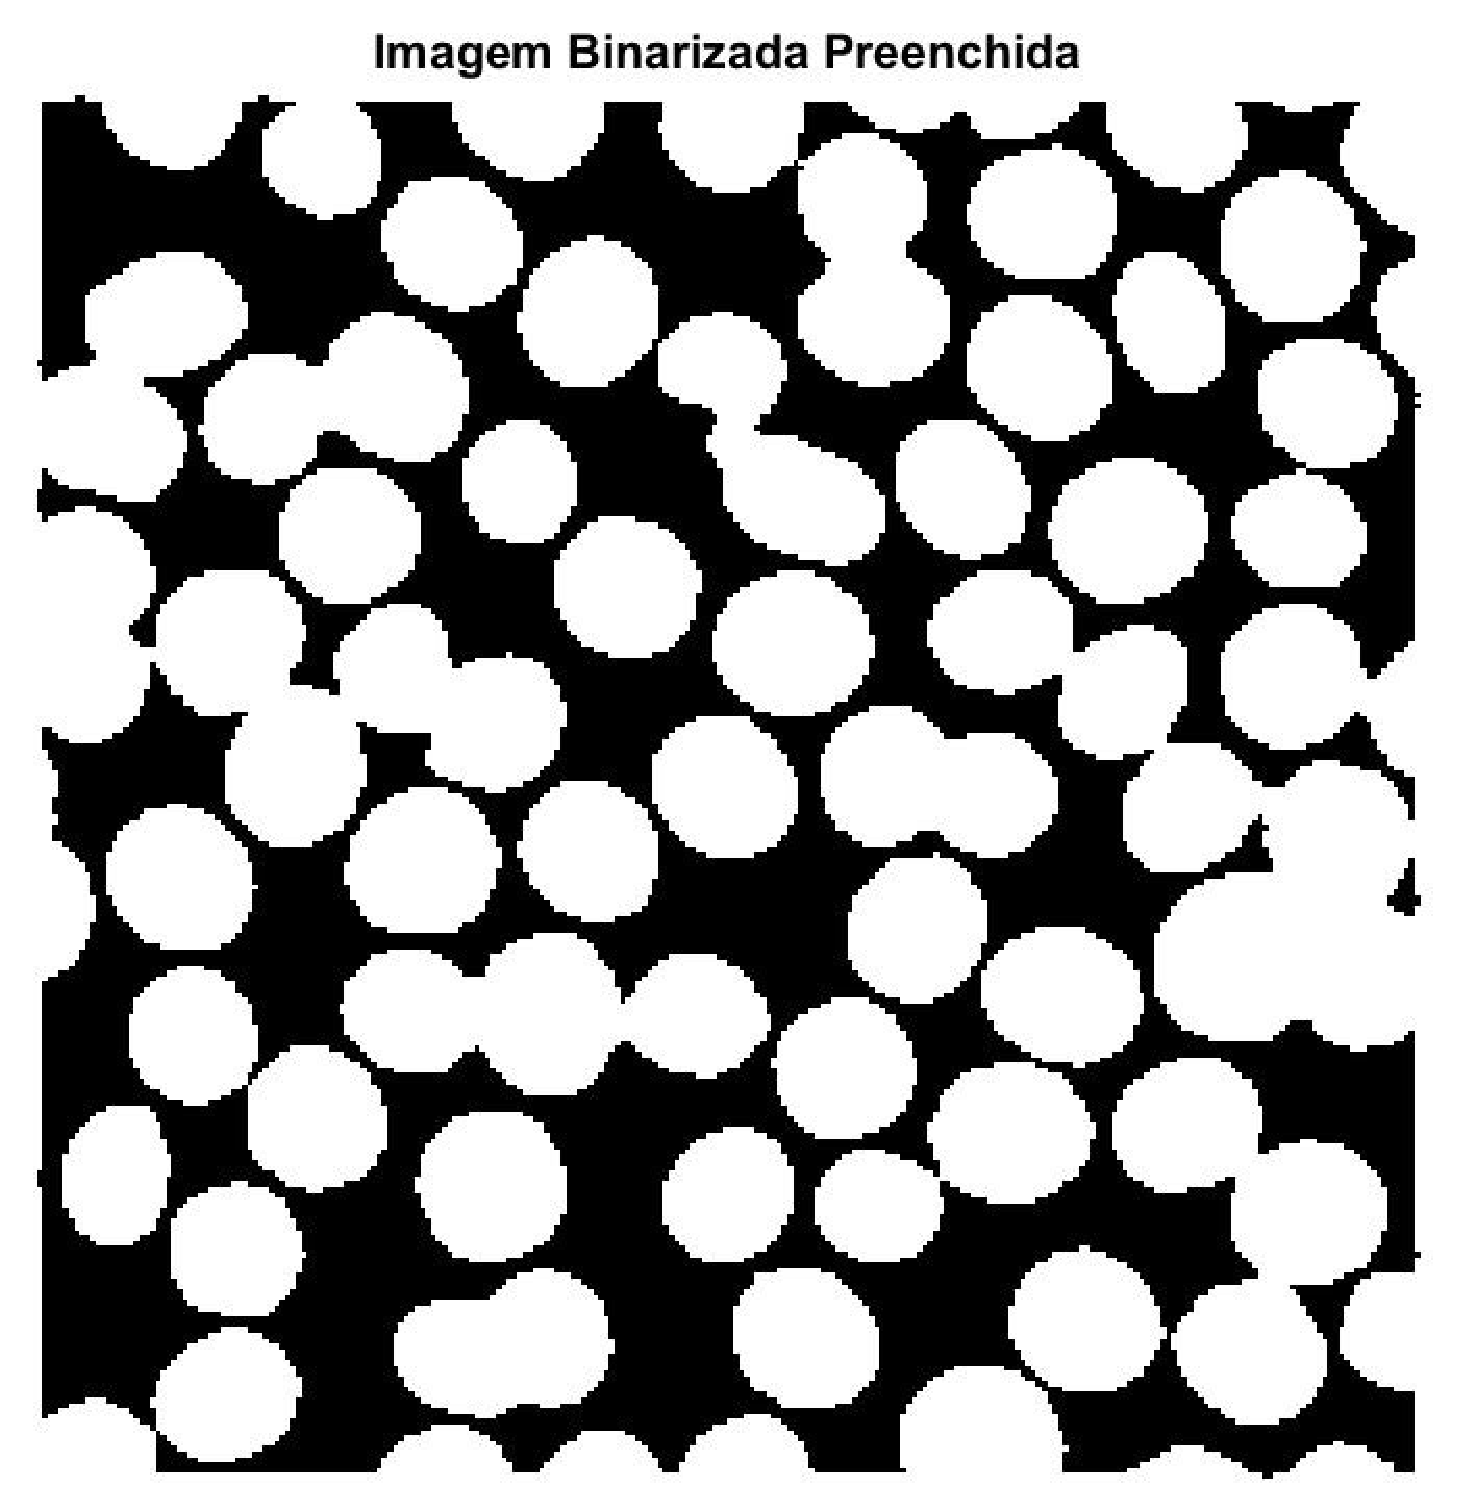
\includegraphics[width = 4.5 cm]{Imagem_Binarizada_Preenchida}
  \caption{Imagem das c\'elulas, ap\'os a binariza\c{c}\~ao e preenchimento dos buracos existentes.}
  \label{fig:prob3.2}
\end{figure}

\begin{figure}[!t]
  \centering
  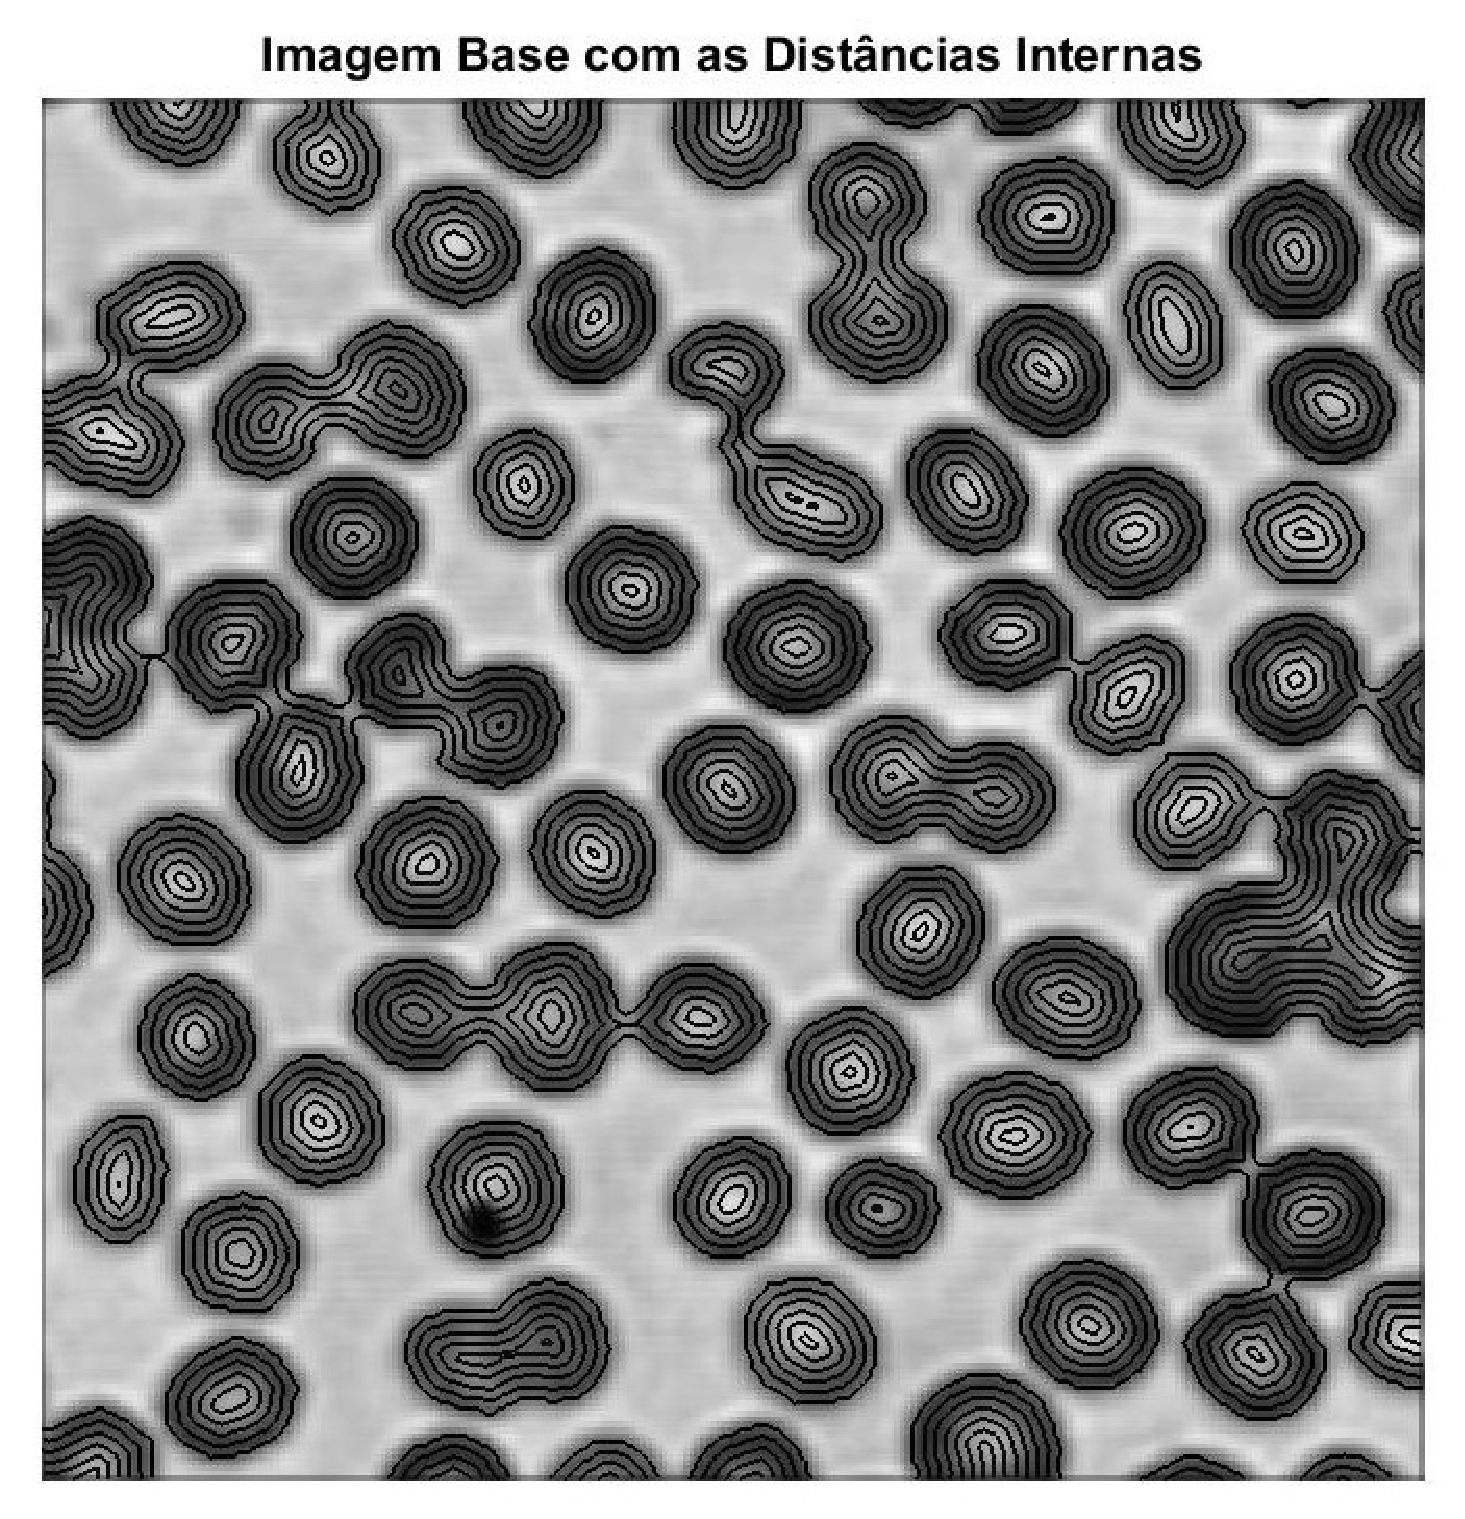
\includegraphics[width = 4.5 cm]{Imagem_Base_com_as_Dist_ncias_Internas_}
  \caption{Imagem das c\'elulas, ap\'os a determina\c{c}\~ao das dist\^ancias e aplicando-as na imagem base.}
  \label{fig:prob3.3}
\end{figure}

\begin{figure}[!t]
  \centering
  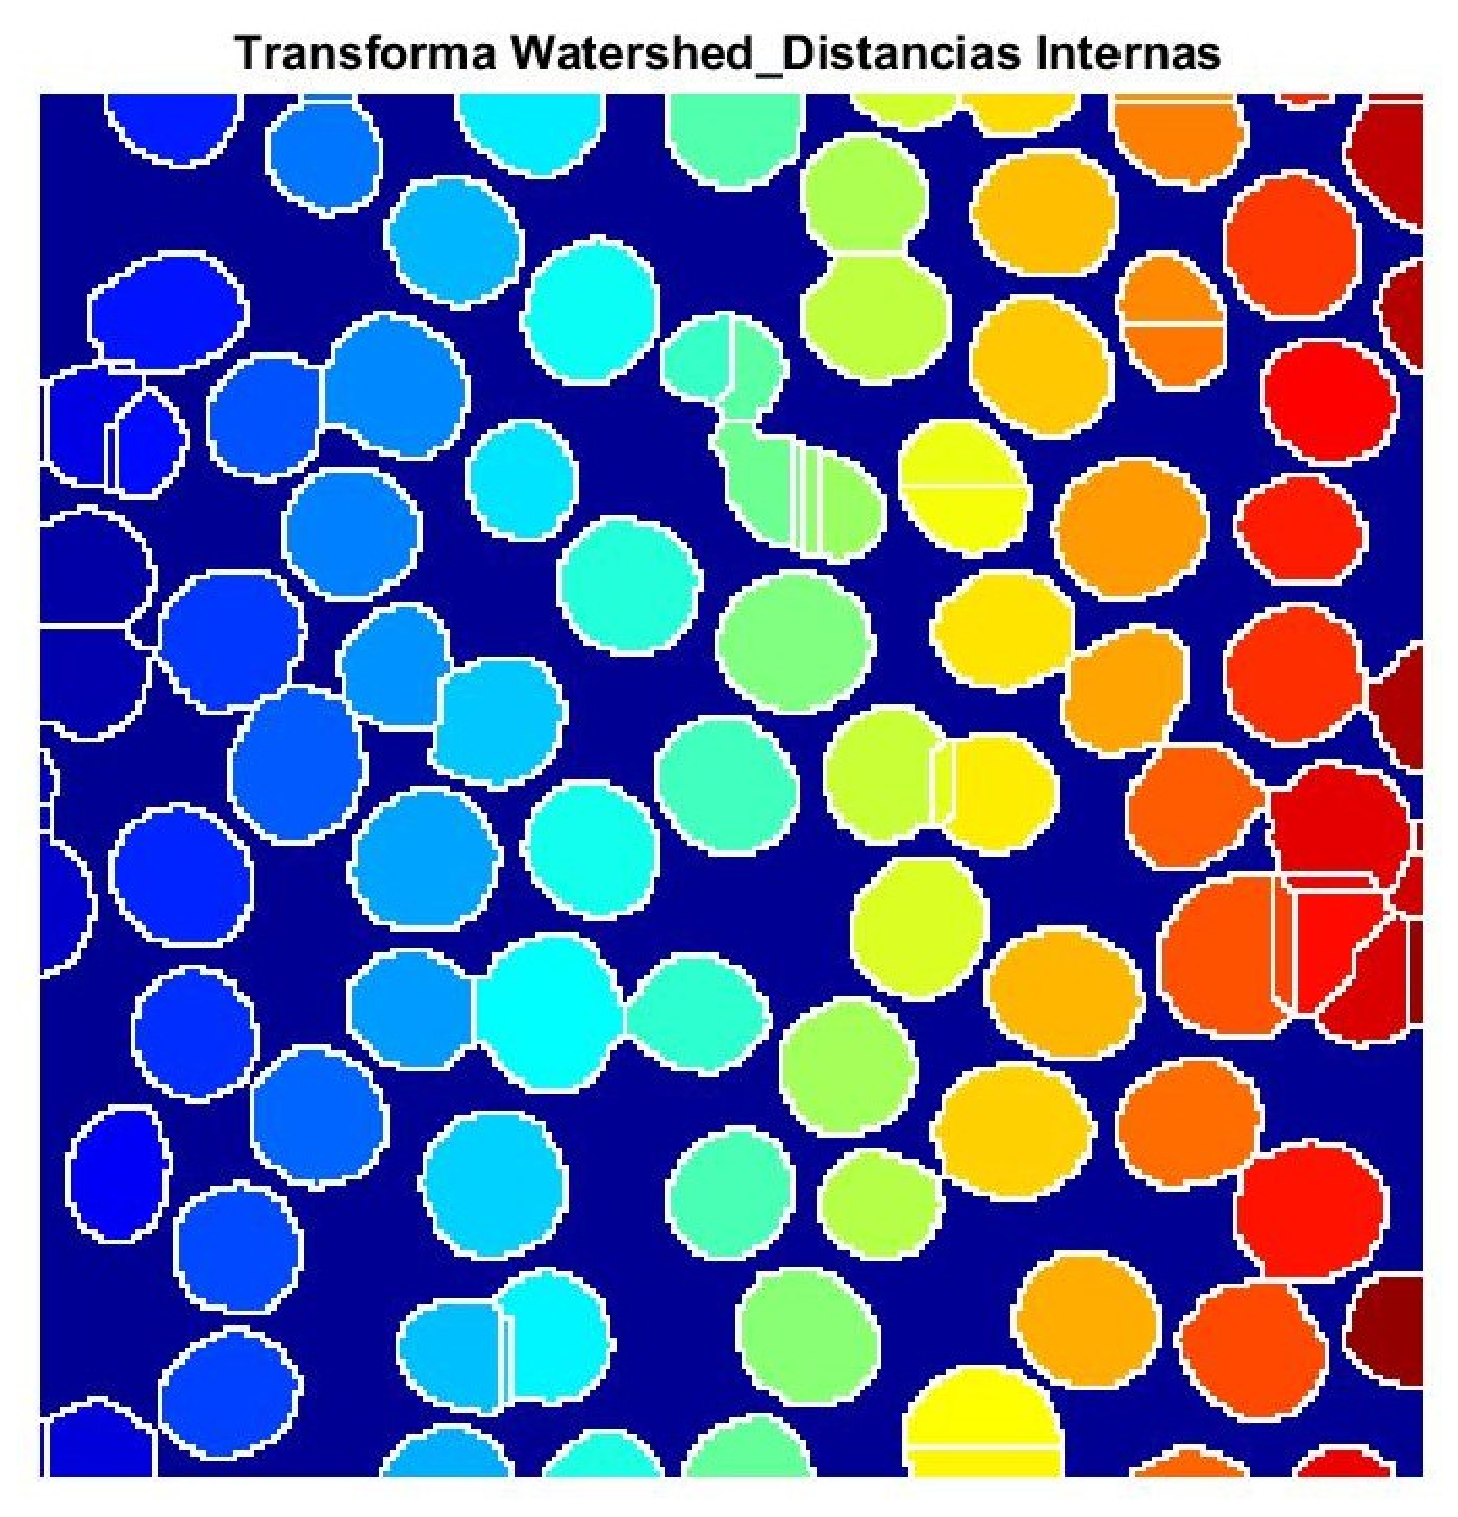
\includegraphics[width = 4.5 cm]{Transforma_Watershed_Distancias_Internas}
  \caption{Imagem das c\'elulas, ap\'os a opera\c{c}\~ao Watershed.}
  \label{fig:prob3.4}
\end{figure}

\begin{figure}[!t]
  \centering
  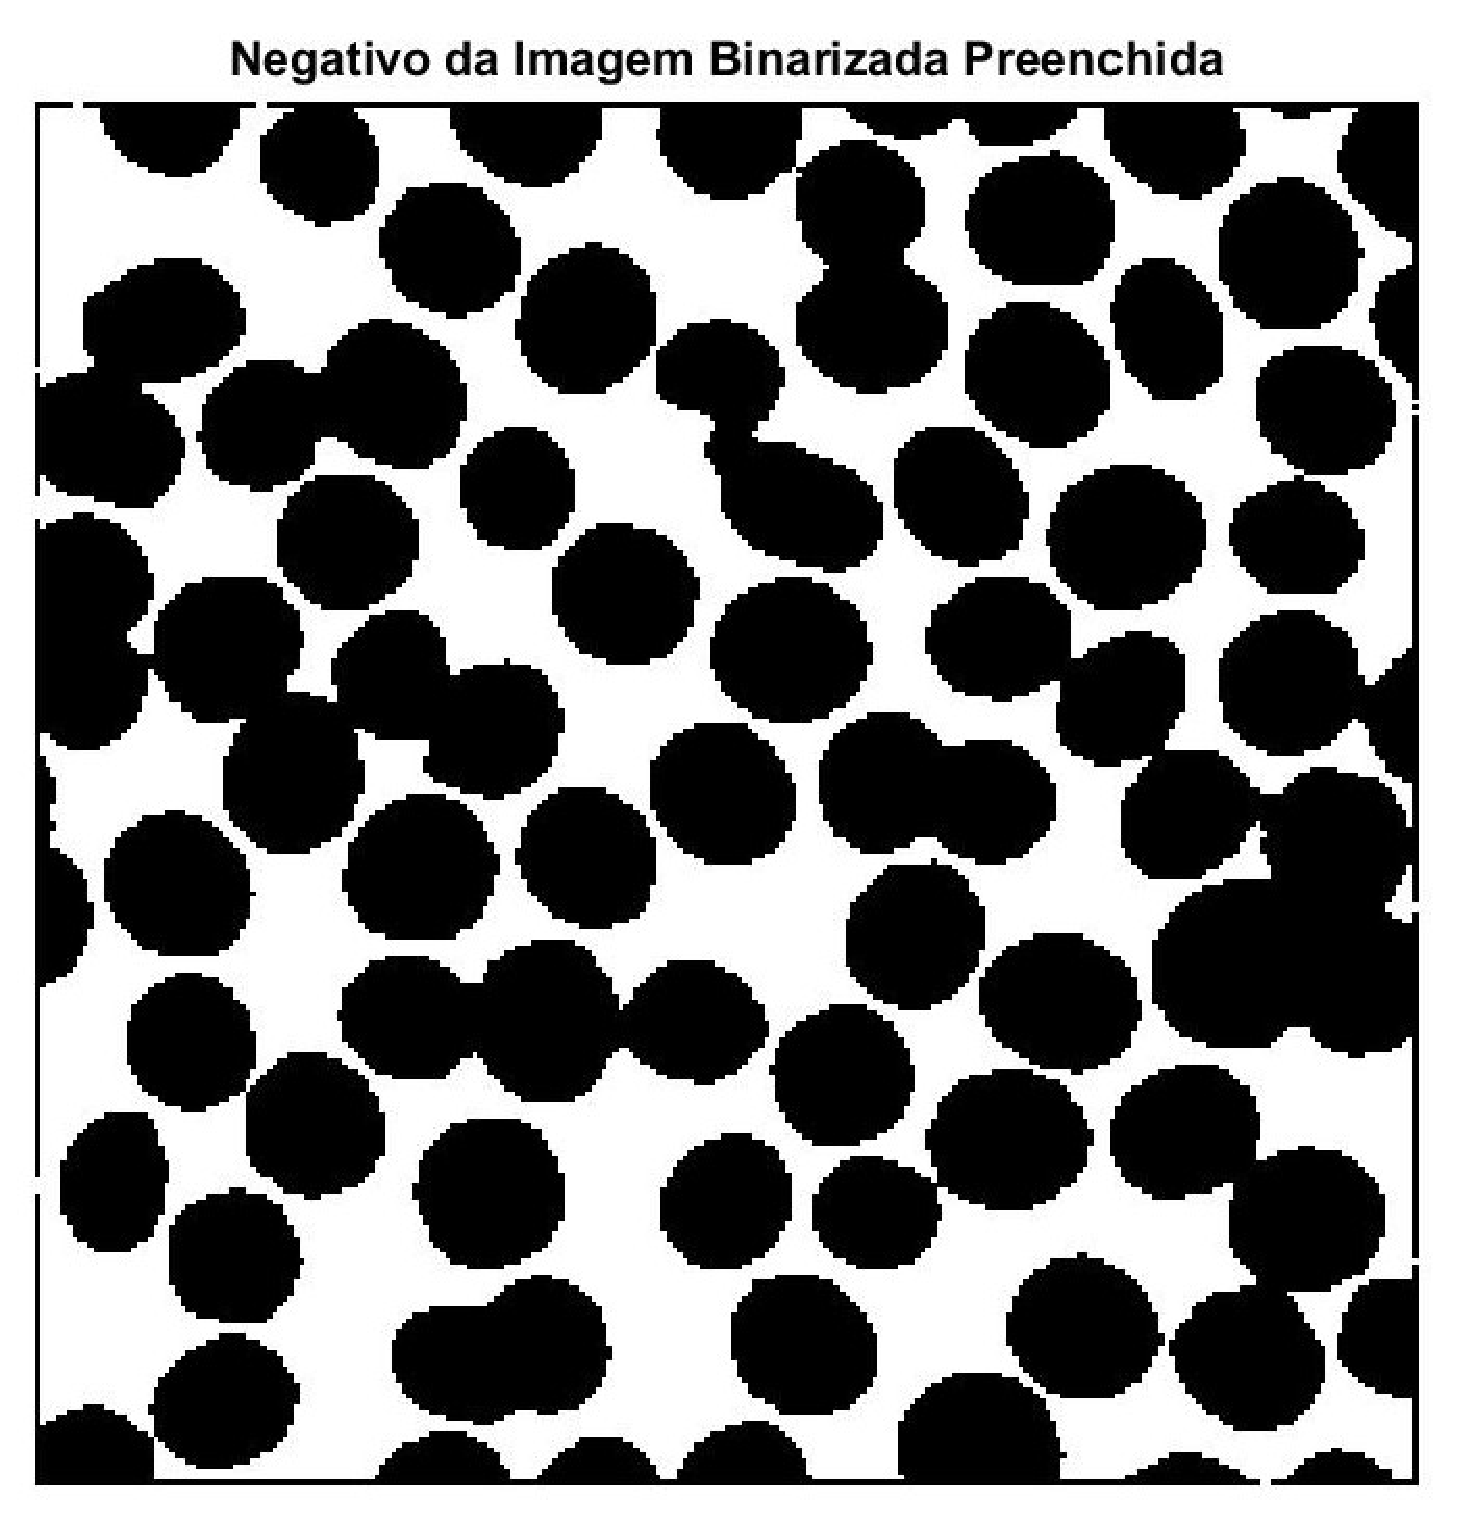
\includegraphics[width = 4.5 cm]{Negativo_da_Imagem_Binarizada_Preenchida}
  \caption{Imagem das c\'elulas, fundo branco e c\'elulas pretas.}
  \label{fig:prob3.5}
\end{figure}



\section{Conclus\~ao}
Com o desenvolvimento do projeto foi poss\'ivel sanar algunas d\'uvidas perante os conte\'udos te\'oricos visto em sala, demonstrando que o objetivo principal foi alcan\c{c}ado. Foram utilizadas as ferramentas disponibilizadas pelo~\textit{MatLab}, que possuem grande poder de atua\c{c}\~ao no processamento de imagens, o que facilitou a fixa\c{c}\~ao dos conceitos, mas \'e esperado que futuramente seja feita uma aplica\c{c}\~ao em~\textit{OpenCV}~\cite{opencv}~(\textit{Open Source Computer Vision Library} ou, em portugu\^es, Biblioteca de Vis\~ao Computacional em C\'odigo Aberto).





% trigger a \newpage just before the given reference
% number - used to balance the columns on the last page
% adjust value as needed - may need to be readjusted if
% the document is modified later
%\IEEEtriggeratref{8}
% The "triggered" command can be changed if desired:
%\IEEEtriggercmd{\enlargethispage{-5in}}

% references section

% can use a bibliography generated by BibTeX as a .bbl file
% BibTeX documentation can be easily obtained at:
% http://www.ctan.org/tex-archive/biblio/bibtex/contrib/doc/
% The IEEEtran BibTeX style support page is at:
% http://www.michaelshell.org/tex/ieeetran/bibtex/
%\bibliographystyle{IEEEtran}
% argument is your BibTeX string definitions and bibliography database(s)
%\bibliography{IEEEabrv,../bib/paper}
%
% <OR> manually copy in the resultant .bbl file
% set second argument of \begin to the number of references
% (used to reserve space for the reference number labels box)
\begin{thebibliography}{1}

\bibitem{Gonzalez}
Gonzalez, Rafael C. e Woods, Richard E.,\emph{Digital Image Processing}, 3$^o$ ed,
Pearson Ed. - ISBN: 9780131687288. 

\bibitem{matlab}
MathWorks. \emph{MATLAB and Simulink for Technical Computing}. Dispon\'ivel em: $https://www.mathworks.com/index.html$, acessado em 2015.

\bibitem{opencv}
Documentation, OpenCV. \emph{Welcome to opencv documentation}. Dispon\'ivel em: $http://docs.opencv.org/index.html$, acessado em 2015.

\bibitem{rosadosventos}
Tr\'iade da Aprova\c{c}\~ao.\emph{N\'iveis de Conhecimento: Por onde come\c{c}ar e at\'e onde voc\^e deve estudar cada assunto?}. Dispon\'ivel em:
$http://triadedaaprovacao.com/niveis-de-conhecimento-por-onde-comecar-e-ate-onde-voce-deve-estudar-cada-assunto/$, acessado em 2015.

\bibitem{down}
4Shared. \emph{Trabalho 2\_IPI\_Rodrigo Guimaraes.zip}. Dispon\'ivel em:
$http://www.4shared.com/zip/vw9zEaLVce/Trabalho2-IPI-RodrigoGuimaraes.html$.

\bibitem{water}
Falc\c{c}\~ao, Alexandre Xavier. \emph{Processamento de Imagens usando Grafos}. Dispon\'ivel em: $http://www.ic.unicamp.br/~afalcao/mo815-grafos/aula6.pdf$, acessado em 2015.





\end{thebibliography}




% that's all folks
\end{document}